\documentclass{article} % \documentclass{} is the first command in any LaTeX code.  It is used to define what kind of document you are creating such as an article or a book, and begins the document preamble
\usepackage{amsmath, amssymb} % For mathematical symbols
\usepackage{geometry} % For page layout
\usepackage{tcolorbox} % For highlighted notes
\usepackage{amsthm} % For theorem environments
\usepackage{enumerate} % For customizing enumeration
\usepackage[super,square]{natbib}
\usepackage{titling}

% Load packages for mathematical typesetting
\usepackage{amsmath}
\usepackage{amssymb}
\usepackage{mathtools}
\usepackage{mathrsfs}
\usepackage{enumitem}
\usepackage{amsthm} 
\usepackage{parskip} 

\usepackage{blkarray} % for block arrays

\usepackage{hyperref} % autoref

\usepackage[demo]{graphicx}
\usepackage{caption}
\usepackage{subcaption}
\usepackage{booktabs}

% Define theorem styles
\theoremstyle{definition}
\newtheorem{definition}{Definition}[section]
\theoremstyle{remark}
\newtheorem*{remark}{Remark}
\theoremstyle{plain}
\newtheorem{theorem}{Theorem}[section]
\newtheorem{corollary}[theorem]{Corollary}
\newtheorem{lemma}[theorem]{Lemma}
\newtheorem{proposition}[theorem]{Proposition}
\newtheorem{claim}{Claim}

% Define an unnumbered theorem environment
\newtheorem*{specialtheorem}{Theorem}
\newtheorem*{specialcorollary}{Corollary}
\newtheorem*{specialproperty}{Property}
\newtheorem*{solution}{Solution}


\title{AI 211 Problem Set Technical Report} % Sets article title
\author{
  Joshua Cantor\\
  \texttt{jzcantor@up.edu.ph}
  \and
  Michael Spencer Quinto\\
  \texttt{maquinto@up.edu.ph}
}
\date{\today} % Sets date for date compiled

\begin{document}
\maketitle % creates title using information in preamble (title, author, date)

\section{Eigenfaces and Face reconstruction}

\subsection{Understanding of the Problem}
    \subsubsection{Motivation}
        Having spent 5 years in the IT industry as professionals, our exposure has predominantly been to general software development and system management. By nature of the work however, we have had very few opportunities to delve into the inner workings and creation of algorithms specifically for computer vision and pattern recognition. As MEngg in AI students, problems such as these allow us to apply and deepen our understanding of machine learning and AI techniques and serve as a foundation to this exciting field that involves a myriad of interesting mathematical concepts.

        Some of these concepts include Singular Value Decomposition (SVD) and Principal Component Analysis (PCA), which are foundational techniques in machine learning, offering crucial insights into data dimensionality reduction, noise reduction, and feature extraction. SVD decomposes a matrix into its constituent singular vectors and singular values, providing a compact representation that captures essential data structures while filtering out noise. PCA, leveraging SVD, transforms data into a new coordinate system where the greatest variances by any projection of the data lie on the first few coordinates called principal components. This transformation is vital for simplifying models, enhancing computational efficiency, and improving visualization of high-dimensional data. For AI practitioners, grasping the intuition and mathematics behind SVD and PCA is essential. It enables them to better understand data structures, apply appropriate preprocessing techniques, and interpret the results of machine learning models more effectively, not to mention, SVD and PCA generally appear in a lot of places where Machine Learning is concerned. Without this foundational knowledge, the use of these techniques could be misapplied or misunderstood, leading to suboptimal models and insights. 
        
        This problem in particular serves as a practical application of the concepts we have learned in Linear Algebra. We have come to a realization of the significant impact that Singular Value Decomposition (SVD) and other linear algebra techniques have on advancements in security, surveillance, and human-computer interaction applications. In particular, the use of SVD in Eigenfaces is noteworthy as it helps in identifying and retaining essential features from a dataset of facial images, thus enhancing the efficiency and accuracy of face recognition systems.

        Furthermore, this problem provides us the opportunity to explore the interdisciplinary nature of AI, combining its mathematical foundations with real-world applications. Understanding how these mathematical concepts are applied in cutting-edge technologies broadens our perspective and prepares us for future challenges in the AI field.

    \subsubsection{Statement of the Problem}
        Face reconstruction through Eigenfaces involves developing a method for efficiently representing and reconstructing human faces using a set of principal components derived from a large dataset of facial images. This approach, rooted in principal component analysis (PCA) and singular value decomposition (SVD), seeks to identify the most significant features (Eigenfaces) that capture the essential variance in the facial images. Each eigenface represents a principal component of the face data, allowing for efficient storage, processing, and reconstruction of facial images. The aim of this approach is to reduce the complexity and computational requirements associated with face recognition and reconstruction tasks, while still retaining the essential characteristics of the faces.

        Understanding and utilizing eigenfaces for face reconstruction is important because it provides a robust method for compressing and reconstructing facial images, which is crucial in various applications such as security, authentication, and human-computer interaction. By focusing on the most significant features that differentiate one face from another, eigenfaces facilitate more efficient and accurate face recognition systems. The significance of this method lies in its ability to handle variations in facial expressions, lighting conditions, and other external factors, making it a powerful tool in the field of computer vision. The ultimate goal of using eigenfaces for face reconstruction is to develop systems that can reliably identify and verify individuals based on their facial features, thereby enhancing the security and effectiveness of biometric identification technologies.

\subsection{Methodology and Snapshots of the Solution}
    \subsubsection{Overview of the Method}
        The program itself is implemented using python. In this problem, Single Value Decomposition (SVD) is applied to a large dataset of facial images (5000 rows) to extract the most dominant correlations between images. The result of this decomposition is a set of eigenfaces that define a new coordinate system, to project the higher-dimensional face-image space to a lower dimension.
   
        Singular value decomposition was also used to compress images by truncating SVD matrices to lower dimensions. Since the components with the most important information are ordered to be in the front, we can use the first \(k\) components to compress an image to reduce not-as-important information in the picture, by truncating the SVD matrices to rank k. As with this specific problem sets and the those that follow, the solutions and analyses were conducted in accordance to guide questions in the problem set.
       
    \subsubsection{Visualizing the Raw Data}
         In order to visualize an individual face image, we need to reshape one row of the matrix \( X \) into a 32x32 matrix and plot it using a grayscale colormap:
        
        \begin{figure}[h!]
            \centering
            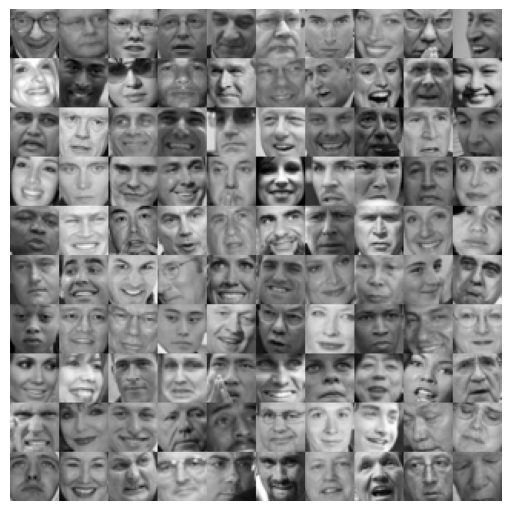
\includegraphics[width=0.42\linewidth]{ps1_eigenfaces/raw_faces.png}
            \caption{First 100 faces of the dataset}
            \label{fig:raw-data}
        \end{figure}

        \autoref{fig:raw-data} represents a montage of 100 grayscale face images arranged in a 10x10 grid, each face reshaped into a 32x32 matrix. Each individual face image highlights various facial structures and expressions, offering a comprehensive overview of the dataset's diversity. Key facial features such as eyes, nose, mouth, and overall face shape are discernible despite the low resolution, illustrating the detailed characteristics that the eigenfaces algorithm would aim to capture and utilize.

        These raw images offer valuable insights into the dataset's quality and variability, essential for understanding the robustness of the eigenface method. The variety in facial expressions, angles, and lighting conditions depicted in the montage underscores the complexity of the data, which the eigenface technique must effectively manage to achieve accurate reconstruction. This initial visualization would help us assess the presence of noise, artifacts, and overall data quality, which are critical factors influencing the performance of the face reconstruction process. Additionally, it provides an intuitive sense of the prominent features that need to be captured, guiding the subsequent dimensionality reduction and reconstruction phases of the eigenface method.

    \subsubsection{Single Value Decomposition}
        Any matrix \(A\) of size \(m \times n\) and rank \(k\) can be decomposed using singular value decomposition (SVD) into a series of three simpler matrices (linear transformations) as follows:
        \[
        A = U \Sigma V^T
        \]
        where:

        \begin{itemize}[label={--}]
            \item \(U\) is an \(m \times m\) orthogonal matrix containing the left singular vectors of \(A\).
            \item \(V\) is an \(n \times n\) orthogonal matrix containing the right singular vectors of \(A\).
            \item \(\Sigma\) is an \(m \times n\) diagonal matrix with the first \(r\) diagonal entries being the positive singular values \(\sigma_1, \sigma_2, \ldots, \sigma_r\), and the rest being zero.
        \end{itemize}
        
        The columns of \(U\) are the eigenvectors of \(AA^T\), and the columns of \(V\) are the eigenvectors of \(A^TA\). The singular values \(\sigma_i\) are the square roots of the non-zero eigenvalues of both \(AA^T\) and \(A^T A\).
        
        In the context of Linear Transformations, each of these matrices, i.e. the SVD components can be interpreted as functions (i.e. takes in a vector and outputs a transformed vector) performing specific linear transformations on vectors:
        \begin{itemize}[label={--}]
            \item Multiplying a vector by the unitary matrices \(U\) or \(V\) rotates the vector without changing its length or the angles between vectors.
            \item Multiplying by the diagonal matrix \(\Sigma\) scales the vectors but does not change their angles.
        \end{itemize}

        Therefore, the process of multiplying a vector \(x\) by the matrix \(A\) involves three steps:
        \begin{enumerate}
            \item Rotate \(x\) using \(V^T\).
            \item Scale the result using \(\Sigma\).
            \item Rotate the scaled vector using \(U\).
        \end{enumerate}

        \begin{figure}[h!]
            \centering
            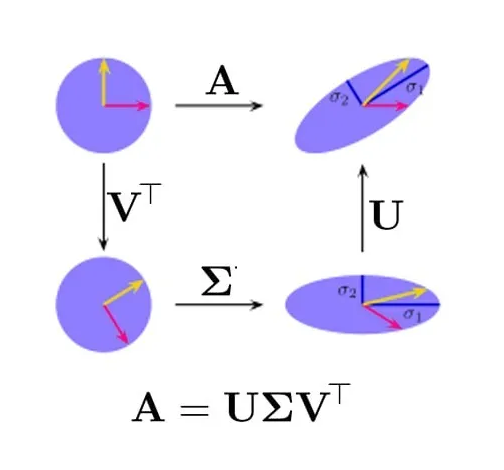
\includegraphics[width=0.35\linewidth]{ps1_eigenfaces/svd.png}
            \caption{Singular Value Decomposition}
            \label{fig:svd-diagram}
        \end{figure}

    We also note that for the general case of rectangular matrices, the $\Sigma$ matrix also performs projection into higher or lower dimensions, depending on whether the matrix is a tall or fat matrix.

    \subsubsection{Eigenfaces}
        Eigenfaces are a set of eigenvectors used primarily in computer vision for the purpose of face recognition. They form a basis set for face images, allowing for a compact representation of a face. If we can find the optimal eigenfaces, we can represent any facial image as a linear combination of these eigenfaces.

        \autoref{fig:svd-diagram} shows a diagram of how SVD decomposes any arbitrary matrix $A$. The row vectors of the matrix \(U\) correspond to these eigenvectors. When we transform the data matrix \(x\) using \(U\), we essentially rotate the original axes to align with the directions of maximum variance in the data. This is the reason why the row vectors of \(U\) define the new axes.

        For the matrix \(A\), the covariance matrix \(C\) can be expressed as:
        \[
        C = \frac{1}{n}AA^T
        \]

        The relation of SVD and Covariance matrix is in the form of matrix \(U\). Notice that \(C = \frac{1}{n}AA^T\). Recall that the SVD of \(A\):
        \[
        A = U \Sigma V^T
        \]
        Consequently,
        \[
        AA^T = U\Sigma V^T V \Sigma^T U^T = U \sigma^2 U^T
        \]

        When we perform SVD on the data matrix \(A\), the columns of \(U\) are the eigenvectors of \(AA^T\), which is the matrix proportional to the covariance matrix of the dataset.

        This is why eigenfaces are associated with the \(U\) matrix in the context of SVD.
        
    \subsubsection{Reduced SVD}
        Reduced SVD (Singular Value Decomposition) can be understood in terms of the four fundamental subspaces of linear algebra shown in \autoref{fig:subspaces}.
        \begin{figure}[h!]
            \centering
            \includegraphics[width=0.50\linewidth]{ps1_eigenfaces/linear-algebra-subspaces.jpg}
            \caption{Four Fundamental Subspaces}
            \label{fig:subspaces}
        \end{figure}

        The dimension of the null space of \(A \in \mathbf{R}^{m,n}\) is related to the number of linearly independent columns that span the null space. For an \(m \times n\) matrix \(A\), the dimension of the null space is \(n - rank(A)\) or \(m-rank(A)\), whichever is larger.
        
        In our case, the Reduced SVD was performed using the \(min(m,n)\) only. \autoref{fig:reduced-svd-diagram} explains the reduction of dimensions while retaining the significant values for \(A\). Where to obtain the reduced SVD from the full SVD, one truncates the matrices $U$, $\Sigma$, $V$ at the $r$-th column or row corresponding to the non-zero singular values. This truncated representation preserves the original matrix's fundamental properties while being more compact and computationally efficient.
        
        \begin{figure}[h!]
            \centering
            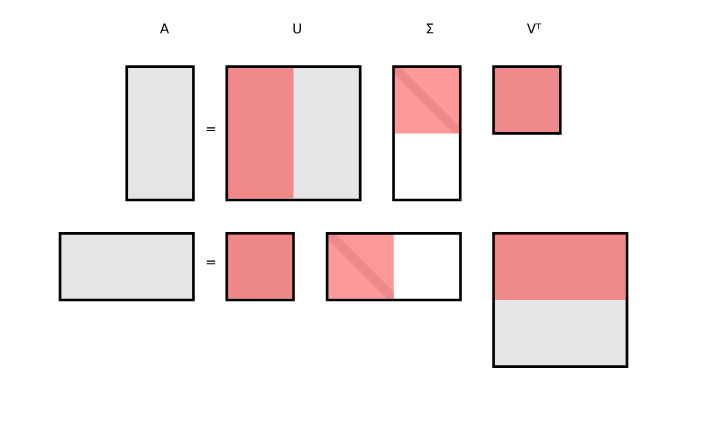
\includegraphics[width=.63\linewidth]{ps1_eigenfaces/reduced_svd.png}
            \caption{Reduced SVD}
            \label{fig:reduced-svd-diagram}
        \end{figure}

        By focusing on \(min(m,n)\) singular values and vectors, reduced SVD implicitly removes the null space from consideration, as it retains only the essential information necessary to reconstruct the matrix.

    \subsubsection{Dimensionality Reduction}
        The primary goal of dimensionality reduction is to reduce the number of features while preserving most of the relevant information. Then, Reduced SVD is one type of Dimensionality Reduction. 
        
        There are many techniques for dimensionality reduction, namely:
        \begin{itemize}[label={--}]
            \item Principal Component Analysis (PCA)
            \item Linear Discriminant Analysis (LDA)
            \item Generalized Discriminant Analysis (GDA)
        \end{itemize}

        The reduced representation should maintain the structure, patterns, and relationships present in the original data. 
        
        This same concept was applied to the algorithm resulting in the Compression and Reconstruction of an image. 

    \subsubsection{Overview of the main Algorithm}
    \begin{verbatim}
    def sv_decomposition(matrix: ndarray, reduced_svd: bool = False):
    \end{verbatim}
    
    \begin{enumerate}
        \item Extract the dimensions, \verb|m| and \verb|n| of the \verb|matrix| with
    
        \begin{verbatim}
        m, n = matrix.shape
        \end{verbatim}
    
        \item Determine the number of singular values to compute based on whether \verb|reduced_svd| is True or False.
         If \verb|reduced_svd| is True, set \verb|s| to the minimum of \verb|m| and \verb|n|. Otherwise, set \verb|s| to the maximum of \verb|m| and \verb|n| with
    
    
        \begin{verbatim}
        if reduced_svd:
            s = min(m, n)
        else:
            s = max(m, n)
        \end{verbatim}
    
        \item Compute \(A^T A\), where \(A^T\) is the transpose of the input matrix \(A\).
    
        \begin{verbatim}
        ATA = np.dot(matrix.T, matrix)
        \end{verbatim}
    
        \[
        A^T A = \begin{bmatrix} a_{11} & a_{12} & \dots & a_{1n} \\ a_{21} & a_{22} & \dots & a_{2n} \\ \vdots & \vdots & \ddots & \vdots \\ a_{m1} & a_{m2} & \dots & a_{mn} \end{bmatrix}^T
        \begin{bmatrix} a_{11} & a_{12} & \dots & a_{1n} \\ a_{21} & a_{22} & \dots & a_{2n} \\ \vdots & \vdots & \ddots & \vdots \\ a_{m1} & a_{m2} & \dots & a_{mn} \end{bmatrix}
        \]

        \item Compute the eigenvalues and eigenvectors of \(A^T A\).
        \verb|eigenvalues_ATA| are the eigenvalues of \(A^T A\), and \verb|V| are the corresponding eigenvectors.



        \begin{verbatim}
        eigenvalues_ATA, V = np.linalg.eig(ATA)
        \end{verbatim}
        
        \[
        A^T A v_i = \lambda_i v_i
        \]

        \item If \verb|reduced_svd| is True, truncate the eigenvalues and eigenvectors to keep only the first \verb|s| values.

        \begin{verbatim}
        eigenvalues_ATA = eigenvalues_ATA[:s]
        V = V[:, :s]
        \end{verbatim}
    
        \item Sort the eigenvalues and their corresponding eigenvectors in descending order of the eigenvalues.

    
        \begin{verbatim}
        sort_desc = np.argsort(eigenvalues_ATA)[::-1]
        \end{verbatim}
    
        \item Apply the sorted indices to reorder the eigenvalues and eigenvectors accordingly.

        \begin{verbatim}
        eigenvalues_ATA = eigenvalues_ATA[sort_desc]
        V = V[:, sort_desc]
        \end{verbatim}
    
        \item Compute the singular values as the square roots of the sorted eigenvalues and form a diagonal matrix \(S\).
    
        \begin{verbatim}
        S = np.diag(np.sqrt(eigenvalues_ATA))
        \end{verbatim}
    
        \[
        \sigma_i = \sqrt{\lambda_i}
        \]
        \[
        S = \begin{bmatrix} \sigma_1 & 0 & \dots & 0 \\ 0 & \sigma_2 & \dots & 0 \\ \vdots & \vdots & \ddots & \vdots \\ 0 & 0 & \dots & \sigma_s \end{bmatrix}
        \]

        \item Compute the inverse of the diagonal matrix \(S\), denoted as \(S^{-1}\).

        \begin{verbatim}
        S_inv = np.linalg.inv(S)
        \end{verbatim}
    
        \item Compute the matrix \(U\) as \(U = AVS^{-1}\).

        \begin{verbatim}
        U = np.dot(matrix, np.dot(V, S_inv))
        \end{verbatim}
    
        \begin{verbatim}
        return U, S, V.T
        \end{verbatim}
    \end{enumerate}

    

\subsection{Results, Analysis and Discussion}
    \subsubsection{Eigenfaces Results}
        \begin{figure}[h!]
            \centering
            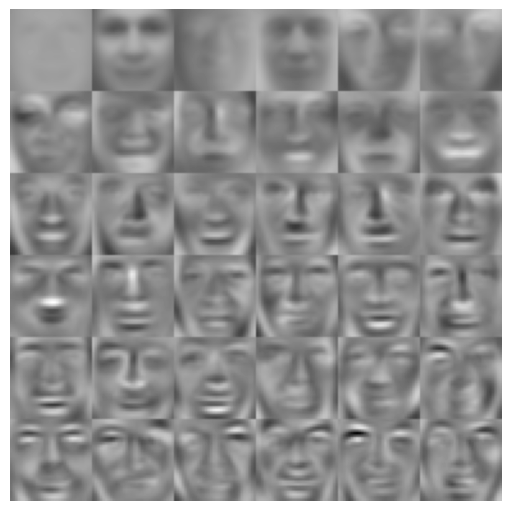
\includegraphics[width=0.36\linewidth]{ps1_eigenfaces/eigenfaces.png}
            \caption{The Singular Values depicted as Eigenfaces}
            \label{fig:eigenfaces-result}
        \end{figure}
        
        \autoref{fig:eigenfaces-result} shows a plot of the first 36 eigenfaces. For the first few pictures shown in the plot, the:
        \begin{itemize}[label={--}]
            \item \textbf{First Eigenface}: Represents the overall average lighting and shadow patterns in the faces.
            \item \textbf{Second Eigenface}: Captures variations in the overall horizontal features of the faces, such as the position of the eyes and width of the face.
            \item \textbf{Third Eigenface}: Highlights the vertical features, such as the position of the mouth and height of the face.
            \item \textbf{Subsequent Eigenfaces}: Capture more localized features such as the presence and shape of facial features (e.g., nose, mouth, eyes) and other finer details.
        \end{itemize}
    \subsubsection{Reduced SVD Results}
        \autoref{fig:log-plots} shows a visualization of the Full vs Reduced SVD logarithmic plots of the singular values \(\sigma\):
        \begin{figure}[h!]
            \begin{subfigure}{.5\textwidth}
                \centering
                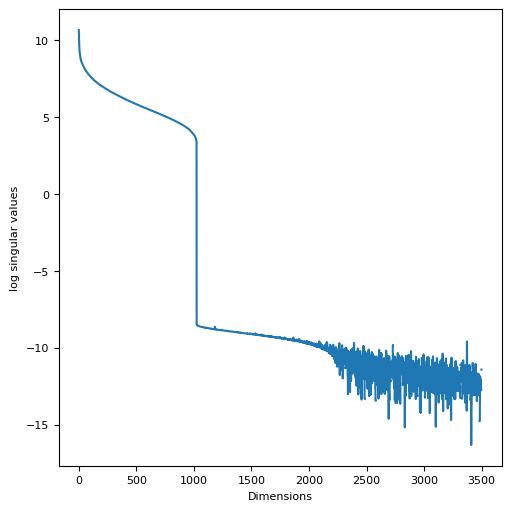
\includegraphics[width=0.85\linewidth]{ps1_eigenfaces/log_singular_values_graph.png}
                \caption{Full SVD}
                \label{fig:full-svd-plot}
            \end{subfigure}%
            \begin{subfigure}{.5\textwidth}
                \centering
                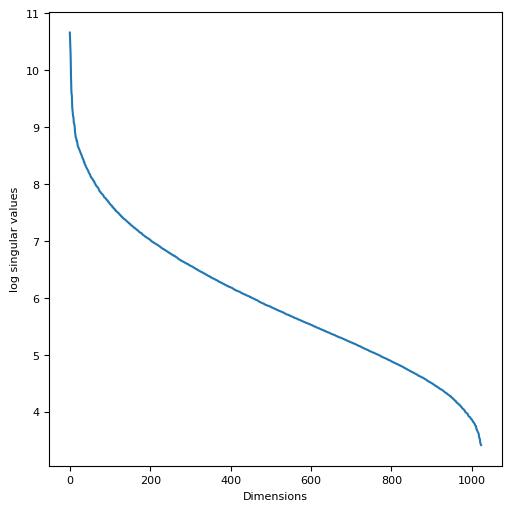
\includegraphics[width=0.85\linewidth]{ps1_eigenfaces/log_singular_values_graph_reducedsvd.png}
                \caption{Reduced SVD}
                \label{fig:reduced-svd-plot}
            \end{subfigure}%
        \caption{Logarithmic Plot of Singular Values}
        \label{fig:log-plots}
        \end{figure}

        Notice how much noise the full SVD plot has. By doing dimensionality reduction, we can remove or truncate null or 0 values from the components of the SVD matrix. 
        
        The rationale for doing dimensionality reduction is that it is "economical" since it reduces the memory/storage of the matrix. Furthermore, it

        \begin{itemize}[label={--}]
            \item Reduces the impact of noise in the data by focusing on the components with the most significant values.
            \item Reduces the computational cost and storage requirements by lowering the number of features.
            \item Simplifies the visualization of high-dimensional data by reducing it to two or three dimensions.
            \item Improves the performance of machine learning algorithms by eliminating redundant and less informative features.
        \end{itemize}
    \subsubsection{Compression using SVD}
        \begin{figure}[h!]
            \centering
            \setkeys{Gin}{width=15.0cm, height=2cm,keepaspectratio}
            \begin{subfigure}{15cm}
                \centering
                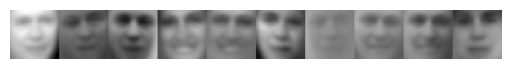
\includegraphics[width=0.55\linewidth]{ps1_eigenfaces/reconstruction1.png}
                \caption*{k = 10}
                \label{enter-label}
            \end{subfigure}
            \begin{subfigure}{15cm}
                \centering
                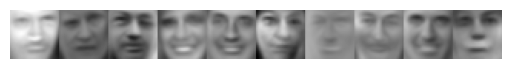
\includegraphics[width=0.55\linewidth]{ps1_eigenfaces/reconstruction2.png}
                \caption*{k = 41}
                \label{enter-label}
            \end{subfigure}
            \begin{subfigure}{15cm}
                \centering
                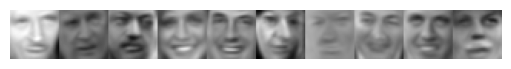
\includegraphics[width=0.55\linewidth]{ps1_eigenfaces/reconstruction3.png}
                \caption*{k = 72}
                \label{enter-label}
            \end{subfigure}
        \caption{Compression}
        \label{fig:face-compression}
        \end{figure}
        \autoref{fig:face-compression} shows a plot of how compression affects the quality of the images and how using even just the first few eigenfaces already gives relatively good results. Compression was achieved in SVD by choosing the first k components from the full set of components. The singular vectors and singular values are ordered in descending order. For this reason, using just the first few singular vectors and singular values will provide enough information for the reconstruction of the image. Moreover, by looking back at the graph of Full vs Reduced SVD, it shows that 1 to 100 dimensions has the biggest singular values.


    \subsubsection{Reconstruction Error}
        \begin{figure}[h!]
            \centering
            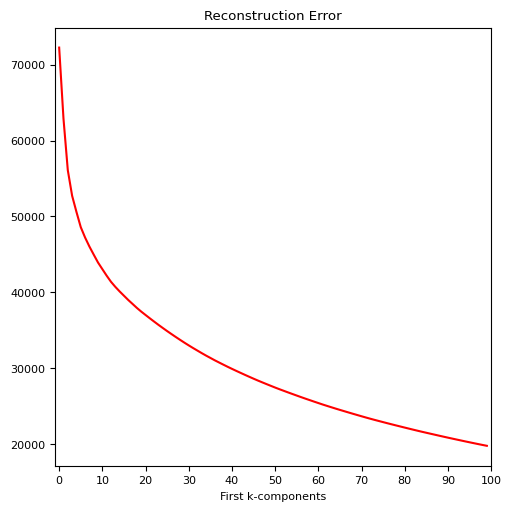
\includegraphics[width=0.6\linewidth]{ps1_eigenfaces/reconstruction_error_norm.png}
            \caption{Reconstruction error from first k-components}
            \label{fig:recon-error}
        \end{figure}
        
        \autoref{fig:recon-error} shows a graph of the reconstruction error against the number of retained singular values \(k\) from the Singular Value Decomposition (SVD).
        The graph exhibits a decreasing trend, denoting that increasing the number of singular values tends to lead to better reconstruction accuracy. Initially, the error is high as fewer singular values capture only the dominant features of the data. However, as \(k\) increases, the error decreases rapidly, capturing more details in the dataset.
        
        At \(k = 20\), the rate of error reduction slows down, indicating diminishing returns, and further increasing \(k\) doesn't significantly improve reconstruction accuracy. This balance between capturing essential features and minimizing error guides in selecting the optimal k, where the curve starts to plateau.

        Understanding this relationship helps in effectively reducing the dimensionality of data while preserving its essential characteristics, crucial for tasks like image or signal reconstruction in various fields such as image processing, data compression, and machine learning.




% ------------------
% ------------------
% ------------------
% ------------------
% ------------------
% ------------------
% ------------------
% ------------------

\pagebreak
    
\section{Nonlinear vs Linearized Least Squares Regression}

\subsection{Understanding of the Problem}

\subsubsection{Motivation}

Least squares regression is a cornerstone of statistical analysis and an essential tool in the field of data science. Its importance extends across numerous disciplines, including biology, economics, engineering, and particularly machine learning. In the context of enzyme kinetics, least squares regression provides a robust method for estimating the parameters of the Michaelis-Menten equation, enabling researchers to gain insights into the catalytic efficiency and substrate affinity of enzymes.

The relevance of least squares regression to modern machine learning cannot be overstated. Many machine learning algorithms, including linear regression, logistic regression, and various neural network training methods, rely on the principles of least squares to minimize error and improve model accuracy, not to mention, it bears several similarities to Gradient Descent and the Backpropagation Algorithm in neural networks. Understanding least squares regression is therefore fundamental for developing and refining predictive models that are used in diverse applications, from medical diagnostics to financial forecasting.

One of the significant aspects of least squares regression is its ability to handle noisy data, which is ubiquitous in real-world scenarios. By minimizing the sum of the squared differences between observed and predicted values, least squares regression effectively reduces the impact of random errors and improves the reliability of the estimated parameters. This attribute is particularly useful in biochemical experiments where measurement inaccuracies are quite common.

Understanding least squares regression is crucial for anyone involved in data analysis, as it forms the basis of more complex machine learning techniques. Its ability to provide reliable parameter estimates in the presence of noise, its historical significance, and its foundational role in modern machine learning make least squares regression an indispensable tool in the arsenal of data scientists and researchers. Thus, it makes sense to spend some time on these methods in order to understand the foundations of Machine Learning.





\subsubsection{Statement of the Problem}

In biochemical kinetics, understanding the relationship between enzyme concentration and reaction velocity is crucial for characterizing enzyme activity. The Michaelis-Menten equation is a fundamental model that describes the kinetics of enzyme-catalyzed reactions. The equation is given by:

\[
v_0 = \frac{v_{max}}{1 + \frac{K_m}{C}},
\]

where \(v_0\) represents the initial reaction velocity, \(v_{max}\) is the maximum reaction velocity, \(K_m\) is the Michaelis constant, and \(C\) is the substrate concentration. The parameters \(v_{max}\) and \(K_m\) are intrinsic properties of the enzyme and are crucial for understanding its catalytic efficiency and substrate affinity.

Typically, \(v_0\) is measured experimentally for various concentrations of the substrate \(C\). To determine the values of \(v_{max}\) and \(K_m\) from experimental data, curve fitting techniques such as least squares regression are employed. Least squares regression is a statistical method used to find the best-fitting curve by minimizing the sum of the squares of the differences between observed and predicted values. In the context of the Michaelis-Menten equation, this involves fitting the nonlinear equation to the experimental data to estimate the parameters \(v_{max}\) and \(K_m\).

There are two primary approaches to fitting the Michaelis-Menten equation: nonlinear least squares regression and linear transformations of the equation followed by linear least squares regression. Nonlinear least squares regression directly fits the original equation to the data, typically using iterative methods like the Gauss-Newton algorithm. Alternatively, the equation can be linearized into forms such as the Lineweaver-Burk, Dixon, and Eadie-Hofstee plots, which transform the nonlinear relationship into a linear one, allowing the use of linear least squares regression to estimate the parameters.

Each method has its own advantages and limitations. Nonlinear least squares regression is often considered more accurate since it fits the original equation directly, but it can be computationally intensive and sensitive to initial parameter estimates. Linear transformations simplify the fitting process but can introduce biases and errors due to the transformation, potentially leading to less accurate parameter estimates.

This study aims to determine the values of \(v_{max}\) and \(K_m\) for a given set of experimental data using both nonlinear least squares regression and various linear transformation methods. By comparing the results obtained from these different approaches, we can evaluate their accuracy and reliability in estimating the kinetic parameters of the enzyme-catalyzed reaction. Understanding these differences is essential for selecting the appropriate method in practical applications of enzyme kinetics analysis.



\subsection{Methodology}

\subsubsection{Nonlinear Least Squares}
Nonlinear least squares regression is used to directly fit the Michaelis-Menten equation to the experimental data. This approach involves minimizing the sum of the squares of the differences between the observed initial velocities (\(v_{0,obs}\)) and the predicted initial velocities (\(v_{0,pred}\)) from the model. The objective function for this minimization is:

\[
S = \sum_{i} (v_{0,obs,i} - v_{0,pred,i})^2.
\]

Given the nonlinear nature of the Michaelis-Menten equation, we employ the Gauss-Newton algorithm, an iterative method, to optimize the parameters \(v_{max}\) and \(K_m\). 

\textbf{Gauss-Newton Method}

The Gauss-Newton method is a modification of the Newton-Raphson method specifically designed for solving nonlinear least squares problems. The core idea is to linearize the nonlinear model around the current estimate of the parameters using a first-order Taylor expansion.

The algorithm can be summarize as follows

\begin{enumerate}
    \item \textbf{Model Linearization}:
    At each iteration, the nonlinear model is approximated by a linear one. For the Michaelis-Menten equation:

    \[
    v_0 = \frac{v_{max}}{1 + \frac{K_m}{C}},
    \]
    
    we define the residuals \(r_i\) as:
    
    \[
    r_i = v_{0,obs,i} - v_{0,pred,i},
    \]
    
    where 
    
    \[
    v_{0,pred,i} = \frac{v_{max}}{1 + \frac{K_m}{C_i}}.
    \]
    \item \textbf{Jacobian Matrix:}
       The Jacobian matrix \(J\) is composed of partial derivatives of the residuals with respect to the parameters. For each data point \(i\):

       \[
       J_{i1} = \frac{\partial r_i}{\partial v_{max}} = -\frac{1}{1 + \frac{K_m}{C_i}},
       \]
    
       \[
       J_{i2} = \frac{\partial r_i}{\partial K_m} = \frac{v_{max} \cdot C_i}{(K_m + C_i)^2}.
       \]
    
       The Jacobian matrix \(J\) thus takes the form:
    
       \[
       J = \begin{bmatrix}
       \frac{\partial r_1}{\partial v_{max}} & \frac{\partial r_1}{\partial K_m} \\
       \frac{\partial r_2}{\partial v_{max}} & \frac{\partial r_2}{\partial K_m} \\
       \vdots & \vdots \\
       \frac{\partial r_n}{\partial v_{max}} & \frac{\partial r_n}{\partial K_m} \\
       \end{bmatrix}.
       \]

    \item \textbf{Parameter Update:}
     The parameters are updated using the Gauss-Newton update rule:

       \[
       \mathbf{\theta}^{(k+1)} = \mathbf{\theta}^{(k)} - (J^T J)^{-1} J^T \mathbf{r},
       \]
    
       where \(\mathbf{\theta}\) is the vector of parameters \([v_{max}, K_m]^T\), \(J^T\) is the transpose of the Jacobian matrix, and \(\mathbf{r}\) is the vector of residuals. This update rule iteratively adjusts the parameters to minimize the sum of squared residuals.
\end{enumerate}


The Gauss-Newton method is particularly useful for nonlinear least squares problems because it leverages the idea of linear approximation to simplify the optimization process. By linearizing the model around the current parameter estimates, the algorithm effectively transforms a nonlinear problem into a series of linear ones, which are easier to solve.

It avoids the need to compute second-order derivatives (as required by the full Newton-Raphson method), reducing computational complexity.
By iteratively refining the parameter estimates, the Gauss-Newton method provides robust solutions even when dealing with complex, nonlinear models.


\subsubsection{Linear Least Squares}
While the Gauss-Newton method provides a direct and accurate way to fit the Michaelis-Menten equation, linear transformations offer a simpler alternative. These transformations convert the nonlinear equation into a linear form, enabling the use of linear least squares regression.

\begin{enumerate}
    \item \textbf{Lineweaver Transformation:}
    \[
       \frac{1}{v_0} = \frac{1}{v_{max}} + \frac{K_m}{v_{max}} \cdot \frac{1}{C}.
    \]
    
       This transformation plots \(\frac{1}{v_0}\) against \(\frac{1}{C}\), yielding a straight line with a slope of \(\frac{K_m}{v_{max}}\) and an intercept of \(\frac{1}{v_{max}}\).

    \item \textbf{Dixon Transformation:}
   \[
   \frac{C}{v_0} = \frac{K_m}{v_{max}} + \frac{1}{v_{max}} C.
   \]

   This transformation plots \(\frac{C}{v_0}\) against \(C\), producing a line with a slope of \(\frac{1}{v_{max}}\) and an intercept of \(\frac{K_m}{v_{max}}\).
   \item  \textbf{Eadie Transformation:}
       \[
   v_0 = v_{max} - K_m \frac{v_0}{C}.
   \]

   This transformation plots \(v_0\) against \(\frac{v_0}{C}\), resulting in a line with a slope of \(-K_m\) and an intercept of \(v_{max}\).
\end{enumerate}


These linear transformations simplify the parameter estimation process, making it accessible and computationally efficient. However, they can introduce biases and errors due to the transformations applied to the data. 

\subsection{Implementation and Snapshots of the Solution}
This section details the implementation of the Least Squares Algorithm as implemented in Python. 

\subsubsection{Nonlinear Least Squares (Gauss - Newton)}
The alogrithm runs inside a for loop depending on the \verb|max_iter| parameter as follows

\verb|for _ in range(max_iter):|
\begin{enumerate}
    \item Calculate $v_{0 predicted}$ with \verb|v0_predicted = michaelis_menten(C, vmax, Km)| based on the current parameters $v_{max}$ and $K_m$.
    \item Calculate Residuals with \verb|residuals_vector = v0_observed - v0_predicted|, where we calculate the differences between observed and predicted initial velocities. This vector represents how far the current model is from the observed data.
    \item Initialize the Jacobian Matrix with: \verb|J = np.zeros((len(C), 2))| where $2$ corresponds to the two parameters $v_{max}$ and $K_m$.
    \item Fill in the Jacobian matrix with the calculated values of the partial derivatives with respect to $v_{max}$ and $K_m$ as follows
    \begin{verbatim}
        J[:, 0] = 1 / (1 + Km / C)            # Partial derivative w.r.t. vmax
        J[:, 1] = -vmax * C / (C + Km)**2     # Partial derivative w.r.t. Km
    \end{verbatim}  
    \item Compute the Gauss-Newton step with \verb|delta = np.linalg.inv(J.T @ J) @ J.T @ residuals_vector| based on the formula $\Delta \theta = (J^T J)^{-1} J^T r$, then update the parameters with \verb|params += delta|.
    \item Finally, we check for convergence with \verb|if np.linalg.norm(delta) < tol: break| where if the change in parameters is smaller than the tolerance, the algorithm has converged, and the loop is broken and the final params should be good enough to approximate the function.
    
\end{enumerate}


\subsubsection{Linear Least Squares}
For Linear Least Squares, since the code for approximating the three linear forms are similar, we will only look at one case, and assume that the same solution generalizes to the other two. Let us consider the \textbf{Lineweaver transformation}.

\begin{enumerate}
    \item Given Data
    \begin{verbatim}
    C = np.array([2.5, 5.0, 10.0, 15.0, 20.0])
    v0_observed = np.array([0.024, 0.036, 0.053, 0.060, 0.064])
    \end{verbatim}
    \item Transform Data for Lineweaver-Burk Plot with
    \begin{verbatim}
    x_lb = 1 / C
    y_lb = 1 / v0_observed
    \end{verbatim}
    This is because $v_0 = \frac{v_{max}}{1 + \frac{K_m}{C}}$ can be linearized into $\frac{1}{v_0} = \frac{1}{v_{max}} + \frac{K_m}{v_{max}} \cdot \frac{1}{C}$, where \verb|x_lb| = $\frac{1}{C}$, the transformed substrate concentrations and \verb|y_lb| = $\frac{1}{v_0}$ the transformed initial velocities.
    \item Create Design Matrix with \verb|X_lb = np.vstack([x_lb, np.ones(len(x_lb))]).T|. This  vertically stacks \verb|x_lb| and a column of ones. The ones account for the intercept in the linear regression model, then we transpose the stacked array to create the design matrix \verb|X_lb|. Each row corresponds to a data point $[x_i, 1]$.
    \item Calculate coefficients using normal equations with 
    \begin{verbatim}
    beta_lb = np.linalg.inv(X_lb.T @ X_lb) @ X_lb.T @ y_lb
    m_lb, c_lb = beta_lb
    \end{verbatim}
    where, in Linear Regression, the coefficients $\beta$ (slope and intercept) can be found using the normal equation $\beta = (X^TX)^{-1} X^T y$. \verb|beta_lb| then contains the coefficients $\beta = [m,c]$ where $m$ is the slope and $c$ is the intercept.
    \item Finally, we estimate the parameters with
    \begin{verbatim}
    vmax_lb = 1 / c_lb
    Km_lb = m_lb * vmax_lb
    \end{verbatim}
    The finaly estimated values for $v_{max}$ and $K_m$ obtained from this should yield an accurate estimate for the Michaelis-Menten equation.
    
    
\end{enumerate}




\subsection{Results, Analysis and Discussion}

\subsubsection{Nonlinear Least Squares(Gauss-Newton)}
\begin{figure}[h!]
    \centering
    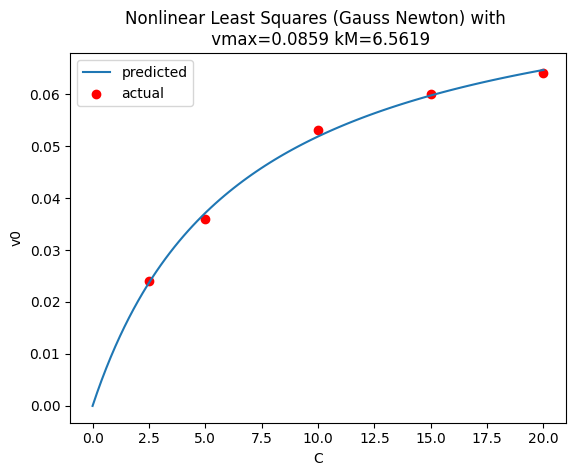
\includegraphics[width=0.60\linewidth]{ps2_nls/01_nls.png}
    \caption{Gauss-Newton Curve Fit vs Actual}
    \label{fig:01_nls}
\end{figure}

\autoref{fig:01_nls} shows a plot of the actual (or observed) data points in red plotted against the curve fit in blue after training using the Gauss-Newton algorithm where after a maximum of 100 iterations, the solution converged to a $v_{max}$ of 0.0859 and a $K_m$ of 6.519 with a sum of squared errors (SSE) of 3.211e-06. Note however that even after just 10 iterations, the algorithm was able to converge to essentially the same parameters with a very similar SSE, indicating that the algorithm was able to approximate the function very well given the observed data.

\subsubsection{Linear Least Squares}

\begin{figure}[h!]
\centering
    \begin{subfigure}{.33\textwidth}
        \centering
        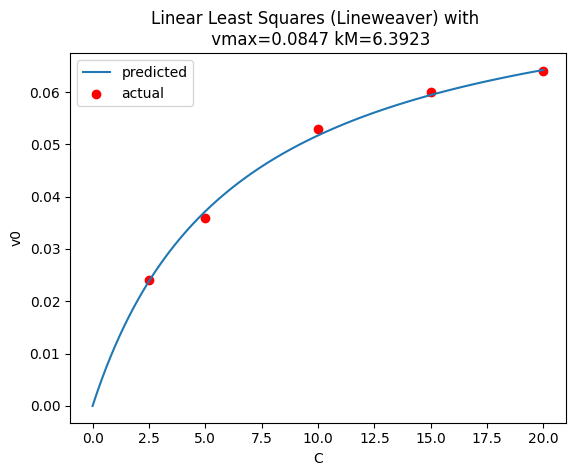
\includegraphics[width=0.99\linewidth]{ps2_nls/02_LLS_lineweaver.png}
        \caption{LLS Lineweaver}
        \label{fig:02_LLS_lineweaver}
    \end{subfigure}
    \begin{subfigure}{.33\textwidth}
        \centering
        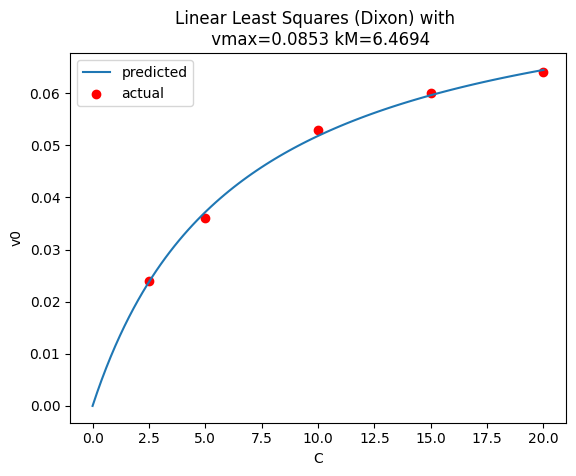
\includegraphics[width=0.99\linewidth]{ps2_nls/04_LLS_dixon.png}
        \caption{LLS Dixon}
        \label{fig:04_LLS_dixon}
    \end{subfigure}%
    \begin{subfigure}{.33\textwidth}
        \centering
        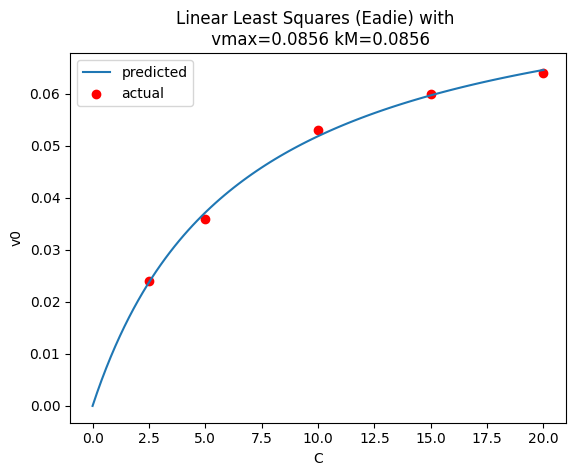
\includegraphics[width=0.99\linewidth]{ps2_nls/03_LLS_eadie.png}
        \caption{LLS Eadie}
        \label{fig:03_LLS_eadie}
    \end{subfigure}%
\caption{Weights applied to example digits}
\label{fig:lls_3_plots}
\end{figure}

\autoref{fig:lls_3_plots} shows the plots of the the solutions obtained using Linear Least Squares when using the three transformed (linearized) equations when plotted against the original nonlinear Michaelis-Menten equation.

\autoref{fig:02_LLS_lineweaver} shows a plot of the predicted vs actual points of the Michaelis-Menten equation when the function's parameters are estimated using Linear Least Squares where the linear equation for the Michaelis-Menten equation is the Lineweaver transformation. Just from the figure, it can be seen that the Linear Least Squares algorithm was able to accurately estimate the parameters that minimizes the squares of the residuals. \autoref{fig:04_LLS_dixon}
 and \autoref{fig:03_LLS_eadie} also show very similar plots with slightly different parameters obtained.


\begin{figure}[h!]
    \centering
    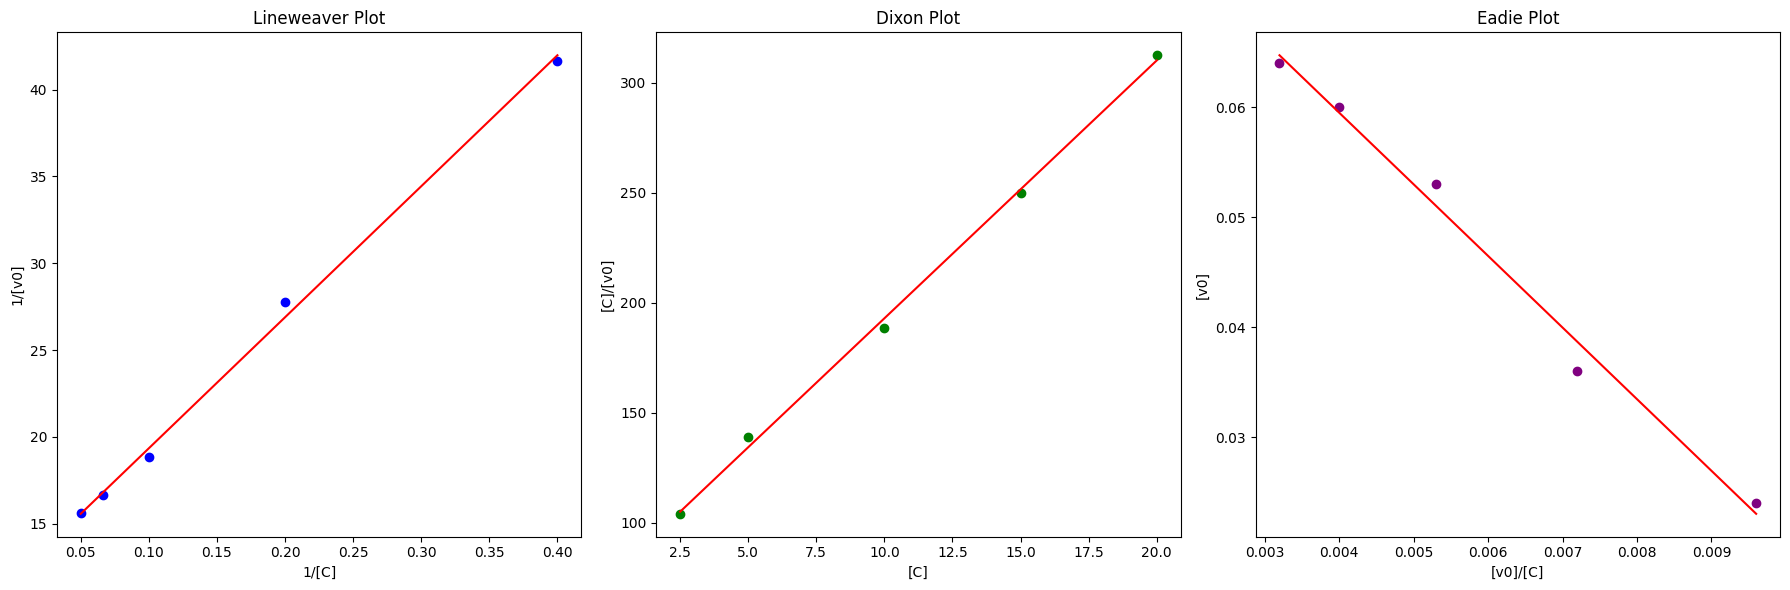
\includegraphics[width=0.99\linewidth]{ps2_nls/05_linear_eq.png}
    \caption{LLS Lineweaver Curve Fit vs Actual}
    \label{fig:05_linear_eq}
\end{figure}

\autoref{fig:05_linear_eq} shows a plot of the three linearized equations where the dots represent the actual observed data and the line represents the best fit curve that minimizes the residuals. Again, in this case, all three plots indicate that the algorithm was able to find an optimum set of parameters to minimize the residuals, thus an accurate esimate of the parameters of the equation.


\subsubsection{Comparison}
\begin{figure}[h!]
    \centering
    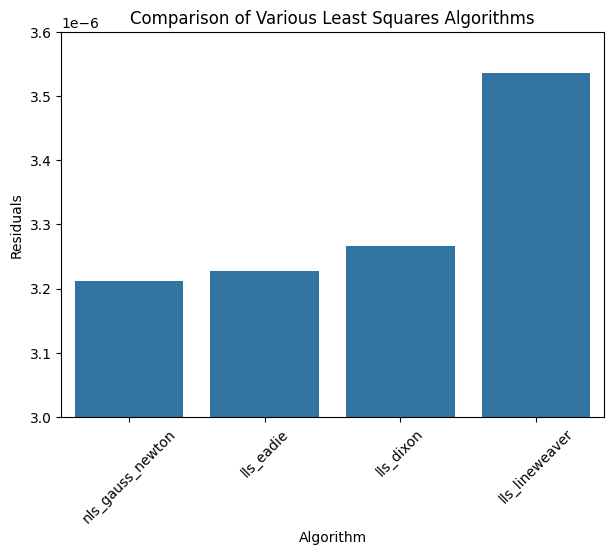
\includegraphics[width=0.60\linewidth]{ps2_nls/06_comparison.png}
    \caption{Comparison of the 4 methods}
    \label{fig:06_comparison}
\end{figure}

\autoref{fig:06_comparison} shows a plot of the square of the residuals for each method where lower is better. Note that the differences between the SSE's for each method is very minute that the we opted to limit the range of the y-axis from 3.0e-6 to 3.6e-6 in order to highlight the minute differences. 

Overall, nonlinear least squares with Gauss-Newton performed the best with an SSE of 3.211e-06, followed by the three linear methods, starting with the Eadie transformation with 3.227e-06, then Dixon with 3.266e-06 and lastly with Lineweaver with 3.535e-06.

\subsubsection{Further Discussion}
The NLS(Gauss-Newton) method directly fits the nonlinear Michaelis-Menten equation. This method minimizes the sum of squared errors (SSE) directly in the space of the original, nonlinear model, providing the most accurate fit for the given data.

As for the three Linear Transformations, the lineweaver transformation linearizes the data but can introduce distortion, especially at low substrate concentrations where measurement errors are amplified.  For Eadie, this transformation also linearizes the data and is less prone to distortion compared to Lineweaver-Burk since it does not involve division by $v_0$. Whereas for Dixon, this transformation involves a combination of the substrate concentration and observed velocity, providing a balance between the two other linear methods.

Linear transformations often involve taking the reciprocal of either the substrate concentration ($C$) or the observed initial velocity ($v_0$). When taking the reciprocal of a small number, any measurement error becomes significantly amplified. For example, if $v_0$ is small $\frac{1}{v_0}$ becomes large, and any small error in $v_0$ translates into a much larger error in $\frac{1}{v_0}$. Furthermore, in linear transformations, the errors are propagated through the transformation equations, potentially distorting the original error structure. For instance, measurement errors in $v_0$ and 
$C$ are transformed in different ways, leading to a misrepresentation of the original data variability.

We can also summarize these statements below.

\textbf{Lineweaver-Burk Transformation}:
   \[
   \frac{1}{v_0} = \frac{K_m}{v_{\max}} \cdot \frac{1}{C} + \frac{1}{v_{\max}}
   \]
   \textbf{Error Amplification}: High
   \begin{itemize}[label={--}]
       \item This transformation involves taking the reciprocal of both \(C\) and \(v_0\).
       \item Small errors in \(v_0\) (especially at low \(v_0\)) get significantly amplified when inverted.
       \item This can lead to a larger SSE because the amplified errors distort the linear regression fit.
   \end{itemize}
   \textbf{Prone to Errors}: Very High
   \begin{itemize}[label={--}]
       \item The amplified errors at low velocities make this transformation highly prone to inaccuracies.
   \end{itemize}\medbreak\medbreak\medbreak\medbreak

\textbf{Eadie-Hofstee Transformation}:
\[
v_0 = v_{\max} - K_m \cdot \frac{v_0}{C}
\]
\textbf{Error Amplification}: Medium
\begin{itemize}[label={--}]
   \item This transformation avoids taking the reciprocal of \(v_0\), reducing the amplification of errors.
   \item It still involves a ratio \(\frac{v_0}{C}\), but this is less prone to error amplification compared to \(\frac{1}{v_0}\).
\end{itemize}
\textbf{Prone to Errors}: Medium
\begin{itemize}[label={--}]
   \item While it still transforms the data, the errors are not as amplified as in the Lineweaver-Burk transformation.
\end{itemize}\medbreak\medbreak\medbreak\medbreak

\textbf{Dixon Transformation}:
\[
\frac{1}{v_0} = \frac{1}{v_{\max}} \left(1 + \frac{K_m}{C}\right)
\]

\textbf{Error Amplification}: Low to Medium
\begin{itemize}[label={--}]
   \item This transformation involves \(\frac{1}{v_0}\) but in a different context than Lineweaver-Burk.
   \item The transformation focuses more on the combination of terms, which can moderate the error amplification compared to simply taking \(\frac{1}{v_0}\) and \(\frac{1}{C}\) directly.
\end{itemize}
\textbf{Prone to Errors}: Medium
\begin{itemize}[label={--}]
   \item This method balances between the extremes of error amplification, but it still suffers from the inherent issues of transforming the data.
\end{itemize}

Again, it should be noted that the result that the NLS algorithm performed better is to be expected as it directly deals with the original equation.
It should be noted however that although not apparent in this specific problems, for some other problems, it might come with a specific set of tradeoffs, which will be summarized below.\medbreak\medbreak\medbreak



\textbf{Nonlinear Least Squares (NLS) with Gauss-Newton}
\textbf{Advantages}
\begin{itemize}[label={--}]
    \item NLS directly fits the nonlinear Michaelis-Menten equation to the data, ensuring that the parameter estimates are as accurate as possible.
    \item By minimizing the sum of squared errors (SSE) in the original data space, NLS avoids the distortions introduced by linear transformations.
    \item NLS can be applied to more complex models beyond the simple Michaelis-Menten equation, accommodating more parameters and intricate relationships.
\end{itemize}
\textbf{Disdvantages}
\begin{itemize}[label={--}]
    \item NLS typically requires iterative optimization, which can be computationally intensive and time-consuming, especially for large datasets.
    \item The Gauss-Newton algorithm can have convergence issues if the initial parameter estimates are not close to the true values.
    \item The performance of the Gauss-Newton algorithm depends on the quality of the initial parameter estimates. Poor initial guesses can lead to non-convergence or convergence to local minima.
    \item  Implementing NLS algorithms like Gauss-Newton requires a good understanding of numerical optimization techniques, making it more complex to code and debug.
\end{itemize}

\textbf{Linear Least Squares (LLS)}
\textbf{Advantages}
\begin{itemize}[label={--}]
    \item LLS methods are straightforward to implement. The linear regression algorithms are well-established and easy to use.
    \item Linear transformations followed by least squares regression are computationally efficient and can handle large datasets quickly.
    \item LLS does not require initial parameter estimates or iterative optimization, avoiding the potential pitfalls of non-convergence associated with NLS methods.
    \item The mathematics behind linear regression is simpler and more intuitive, making it easier to understand and explain the results.
\end{itemize}
\textbf{Disadvantages}
\begin{itemize}[label={--}]
    \item Linear transformations (such as Lineweaver-Burk) can amplify measurement errors
    \item Linear transformations are specific to particular models (e.g., Michaelis-Menten) and cannot easily be extended to more complex or different types of nonlinear models.
    \item Transforming the nonlinear equations like the Michaelis-Menten equation into a linear form can distort the true relationship between the parameters.
\end{itemize}

In the specific case of this problem, it should be noted that using either NLS or LLS leads to highly accurate results, as such, for this specific problem, it doesn't matter that much which method we go with. For more complex problems however, it would be worth it to take into consideration the advantages and disadvantages discussed above, but the main gist is, go for NLS if accuracy is a concern, while go for LLS if speed is a priority.


% ------------------
% ------------------
% ------------------
% ------------------
% ------------------
% ------------------
% ------------------
% ------------------








\pagebreak

\section{MNIST Handwritten Digit Classification Using ANN}

\subsection{Understanding of the Problem}

\subsubsection{Motivation}
Neural Networks have become ubiquitous in the age of modern machine learning and come with all sorts of differing architectures such as CNNs, RNNs, Transformers, etc. At the core however, these different ANN architectures share the same underlying core principles albeit with slightly different implementations depending on their specific specialty domains. For example, the earliest form of neural networks only involved feedforward neural networks such as the Multilayer Perceptron (MLP). Other forms include time-delay, recurrent neural networks, etc. which is in contrast to the unidirectional MLP. Even if these models might be used for vastly different domains, it remains that all of these different neural network architectures share the same mathematical foundations, and that alone makes a study of the math behind it worthwhile.

An understanding of Linear Algebra is critical as neural networks typically involve the maniuplation of large amounts of matrices. Differential Calculus provides a glimpse into how minute different changes in weights affect other components of a neural network (such as the cost function) through the chain rule. Probability theory helps in understanding the stochastic nature of neural network training and in designing models that can generalize well from training data to unseen data.

Given how ubiquitous and powerful Neural Networks are in Machine Learning, a deep understanding of the inner workings of Neural Networks has proven to be a very powerful asset in the training of these models, especially when problems involve non-trivial and fairly uncommon levels of customization. In addition to this, learning the foundations provides a deep comprehension of how these models learn from data, enabling practitioners to debug, optimize, and enhance their performance effectively. Without this knowledge, one might rely solely on trial-and-error, which can be inefficient and suboptimal.

Furthermore, a solid grasp of backpropagation, the algorithm used to train neural networks by minimizing a loss function, allows practitioners to understand how gradient-based optimization methods adjust weights and biases. This understanding is essential for addressing issues such as vanishing and exploding gradients, which can significantly impact the training process. Moreover, insights into the mathematical foundations and mechanisms of neural networks foster innovation, as researchers can design new architectures, activation functions, and learning algorithms tailored to specific tasks or challenges. In essence, mastering the theory behind neural networks and backpropagation not only equips one with the tools to effectively use these models but also empowers them to push the boundaries of machine learning and artificial intelligence.

\subsubsection{Statement of the Problem}
This paper focuses on the relatively simple Multilayer Perceptron as it provides an opportunity to dive into the basics of how neural networks "learn" associations. 

The problem involves handwritten digit recognition on the MNIST dataset where the dataset is composed of 5000 handwritten digits as 20x20 pixels. The task of the neural network is then to find the optimal set of weights and biases that minimize the loss function given these 5000 digits as input and their class labels for the calculation of the loss function. The problem can then be framed as a multiclass classification problem where the Neural Network is fed a series of 400 pixel values and its corresponding label, then the task of the network is to find a set of weights and biases such that when a training pattern is fed, the neurons in the output layer should correspond to the training label.

\subsection{Methodology}

\subsubsection{Overview of the Method}
The neural network is implemented in Python as a class to enable the creation of multiple instances with different hyperparameters. Optimization of the Neural Network is done using mini-batch Stochastic Gradient Descent where for each epoch, the full set of the training data is split into mini-batches before the forward passes are performed. The gradients and change in weights are then calculated using the Backpropagation algorithm where the local gradients and change in weights are calculated from the output layer, then proceeding backwards back to the input layer through the application of the chain rule from Calculus.

The next subsections will be detailing the steps involved in the calculation of the weight updates, including forward and backpropagation.

\subsubsection{Neural Network Model}
Consider a neuron $j$ in layer $l$ where the previous neurons are indexed by $i$ and the next neurons are indexed by $k$.

The input layer of the model takes in all of the 400 features (pixels) per dataset, which is then passed to the hidden layer until they reach the output layer where the multilabel classification happens. The activations for each layer is calculated as follows

\begin{equation}\label{net_int}
	{v_j(n)}^{l} = \sum_{i=0}^{m} {w_{ji}}^{l} {y_i}^{l-1}
\end{equation}

where $n$ is the sample number (or the nth training pattern), $l$ is the layer number, $l-1$ indicates a preceding layer, $w$ is one of the specific weights attached to the neuron, $y$ is the activation (or input in the case of the first hidden layer) from the previous layer and $v$ is the net internal activity. 

The activations per neuron are then calculated as follows

\begin{equation}\label{activ}
	{y_j}^{l} = \varphi({v_j}^{l})
\end{equation}

where $\varphi$ is the activation function. The specific activation functions used in this paper is sigmoid.

In order to indicate how well the network is performing, a loss function is then introduced and is defined as follows

\begin{equation}\label{cost}
	\mathcal{L} = \frac{1}{2} \sum_{j \in C} \left( d_j - y_j \right)^2
\end{equation}
where $\mathcal{L}$ is the cost function for the specific training pattern, $d_j$ is the desired output for class $j$ and $y_j$ is the predicted output and $C$ is the set of all output neurons of the network. In order to take into account the full cost through all training patterns however, we take the average across all training examples as follows

\begin{equation}\label{avg_cost}
	\mathcal{L}_{av}  =  \frac {1}{N}  \sum _ {n=1}^ {N}  \mathcal{L} =  \frac {1}{2N}  \sum _ {n=1}^ {N}  \sum  {e_{j}}^{2}
\end{equation}

$\mathcal{L}_{av}$ is the average cost across all training examples and will serve as a metric for how well our network is performing at a specific point in time with a specific set of weights and biases, and $e_j = d_j-y_j$.

In order then to improve the performance of the network, we aim to minimize the cost function, which can be imagined as a hypersurface in hyperdimensional space. This is where several key ideas come into play, starting with the idea of the gradient of the function, which mathematically indicates the direction of steepest ascent of a function. In order then to obtain a local minima of a function, we take small steps in the direction of the negative of the gradient vector. The process of taking small steps in the direction of the negative of the gradient vector is termed appropriately as Gradient Descent.


For neural networks in particular, the process of computing the specific set of partial derivatives is known the as Backpropagation algorithm and lies at the heart of every modern neural network and all of its derivative architectures.


Mathematically, the gradient vector represents the full set of first-order partial derivatives with respect to each weight and bias and is defined as follows

\begin{equation}\label{grad_output}
	\frac{\partial \mathcal{L}}{\partial w_{j i}}=\frac{\partial \mathcal{L}}{\partial e_j} \frac{\partial e_j}{\partial y_j} \frac{\partial y_j}{\partial v_j} \frac{\partial v_j}{\partial w_{j i}}
\end{equation}

where we note that neural networks as simply a long chain of functions composed one on top of the other until they reach the output layer. In order then to calculate the partials derivatives with respect to each weight, we apply the chain rule from calculus where we start at the point where the function is computed (at the output layer), then proceed layer by layer backwards, unpacking each function composition in order to calculate the needed change in weights, again, this process is know as the Backpropagation algorithm.

\autoref{grad_output} can be rewritten as

\begin{equation}\label{grad_output_simp}
	\frac{\partial \mathcal{L}}{\partial w_{j i}}=-e_j \varphi^{\prime}\left(v_j\right) {y_i}^{l-1}
\end{equation}

after taking into account the specific functions used in the partial derivatives, where $\varphi^{\prime}$ is the derivative of the activation function.

It should be noted however that during the calculations of the gradient, a specific portion of the calculations from the current layer can be reused in the calculations for the previous layer, this is known as the local gradient or the local error for a particular neuron and is defined as follows

\begin{equation}\label{local_error_output}
	\delta_j(n)=e_j \varphi^{\prime}\left(v_j\right)
\end{equation}

for output neurons, and


\begin{equation}\label{local_error_hidden}
	\delta_j(n)= \varphi^{\prime} (v_j) \sum_k {\delta_k}^{(l+1)} {w_{kj}}^{(l+1)}
\end{equation}

for hidden neurons. For hidden neurons, in the case where they are connected to more than one neuron to the next layer, this results in the case where they can influence the cost function through more than one neuron. This effect is taken into account by the summation term in the equation.


Since the adjustment of weights is directly proportional to the gradient of the cost function, we can then calculate for the specific weight changes needed for each weight and bias as follows


\begin{equation}\label{weight_update}
	\Delta {w}_{ji}(n) = -\eta \frac{\partial \mathcal{L}}{\partial w_{ji}}
\end{equation}

where $\eta$ is the learning rate. 

We can also rewrite the formula for the change in weight as follows


\begin{equation}\label{final_weight_update}
	\Delta {w}_{ji} = \eta {\delta_j}^{(l)} {y_i}^{(l-1)}
\end{equation}

Finally, the formula for the weight update is as follows

\begin{align*}
    {w_{ji}^{(l)} (n+1)} & =  {w_{ji}^{(l)} (n)} + \Delta {w}_{ji} \\
    & = {w_{ji}^{(l)} (n)} + \eta {\delta_j}^{(l)} {y_i}^{(l-1)} \\
\end{align*}

\subsection{Implementation and Snapshots of the Solution}

This section details the implementation of the Neural Network as implemented using Python. The algorithm itself is implemented without any external libraries except for numpy, while several methods from sklearn are imported only for the purposes of test-validation splits and the calculation of performance metrics.

\subsubsection{Initialization of Weights}
Weights are initialized during the creation of the Multilayer Perceptron class (MLP) with a standard normal distribution.

During the initialization of the MLP class, the sizes of the layers are passed as arguments into the class constructor 
\begin{verbatim}
    network = MLP(layer_sizes=[400, 25, 10])
\end{verbatim}
as a list of the number of neurons per layer. Then during the initialization of the actual weights, we add one more weight per neuron to account for the bias with
\begin{verbatim}
    self.weights = [
        np.random.randn(right_layer_neurons, left_layer_weights + 1)
        for (right_layer_neurons, left_layer_weights) in zip(
            self.layer_sizes[1:], self.layer_sizes[:-1]
        )
    ]
\end{verbatim}
as the bias can be treated as a trainable weight with a constant input of 1.

\subsubsection{Stochastic Gradient Descent (SGD)}
Although the theoretical most accurate way of calculating the gradient would be to run through all the training examples, then compute the average of the change in weights per neuron across all training examples. This proves to be fairly computationally-expensive task, especially for very large datasets involving multiple layers.

Stochastic Gradient Descent is a technique applied in Machine Learning wherein instead of looping through all of the training examples for each epoch before updating the weights, we instead partition the entire training set into subsets called mini-batches. We then loop through all of the training patterns contained within the mini batch, then update the weights after the entire mini-batch has been fully processed.

Mini-batch SGD can be visually interpreted as taking small but highly accurate steps downwards the loss function hypersufrace. This is in contrast to SGD which can be interpreted as taking larger less accurate downward steps which usually helps training proceed much faster.

Below is a rough overview of the steps used in the algorithm implemented in Python

\begin{enumerate}
    \item Create the MLP instance, for example: \verb|network_a = MLP(layer_sizes=[400, 25, 10]|.
    \item MLP class constructor initializes the weights.
    \item call the \verb|SGD_fit| method.
    \item The \verb|SGD_fit| method does a loop from 1 to N epochs.
    \item For each epoch, the training data is randomly shuffled then split into mini-batches
    \item Each mini-batch is processed with \verb|self.process_mini_batch| (a method inside the \verb|MLP| class)
    \item \verb|self.process_mini_batch| loops through each of the training examples inside the mini-batch as follows. First, before going through the loop, we initialize a list that would contain the calculated delta weights per training example in the mini-batch, \verb|mini_batch_deltas = []|, then the loop goes: \\
    \verb|for y_train, X_train in mini_batch:|
    \begin{enumerate}
        \item \verb|y_out = self.forward(X=X_train)|: Perform forward propagation on \verb|X_train|, note that \verb|X_Train| is a single training example from the mini-batch. The result should be the output activations of the last neuron, let's call this \verb|y_out|.
        \item \verb|Delta_weights = self.backward(y_train=y_train, output_activatons=y_out)|: Perform backpropagation on \verb|X_train|. The result is a list of numpy arrays corresponding to the change in weights where each of the elements of the list correspond to the change in weights per layer.
        \item \verb|mini_batch_deltas.append(Delta_weights)|: Append the change in weights to the list \verb|mini_batch_deltas = []|.
        \item \verb|mini_batch_deltas| now contains a list of lists of weight changes per layer, and can be visualized as follows
        \begin{verbatim}
            mini_batch_deltas = [
                [DW1, DW2, ..., DW_N],
                [DW1, DW2, ..., DW_N],
                [DW1, DW2, ..., DW_N],
                ...
                [DW1, DW2, ..., DW_N],
            ]
        \end{verbatim}
        where each \verb|DW| is a \verb|numpy| array corresponding to the change in weights per layer. For example, \verb|DW1| would be the change in weights for the first hidden layer, while \verb|DW_N| for the output layer. Also note that per row, the \verb|DW|'s almost certainly do not have the same shapes.

        In order to calculate the average of the change in weights per layer, all \verb|DW1|'s and the other corresponding \verb|DW_N|'s must be placed into the same list. This is done by transposing the list using the \verb|zip| function, then converting each of the rows into numpy arrays (at this point, each row's \verb|ndarray| elements have the same dimensions because they correspond to the change in weights for the same layer, but for different training patterns). 
        
        \item The average change in weights per layer can then be calcualted with
        \begin{verbatim}
        Delta_weights_means = [
            np.mean(layer_deltas_in_mini_batch, axis=0)
            for layer_deltas_in_mini_batch in transposed_mini_deltas
        ]
        \end{verbatim}
        The resulting \verb|Delta_weights_means| list contains numpy arrays of the same shape as \verb|self.weights|.
        \item Update the weights based on the average weight changes across the mini-batch with
        \begin{verbatim}
        self.weights = [weight + Delta 
            for weight, Delta in zip(self.weights, Delta_weights_means)
        ]
        \end{verbatim}
    \end{enumerate}
\end{enumerate}



\subsubsection{Backpropagation (deeper dive)}
\begin{enumerate}
    \item Recall that for a neuron $j$ in the output layer, the error, $e$ is calculated as $e_j = d_j - y_J$. This can be calculated as a vector by one-hot encoding the desired activations for the output neurons (stored inside \verb|one_hot|) and subtracing it by the activations obtained from the forward propagation step.
    \item We then loop through all of the activations per layer, starting from the output layer, moving backwards. Note that each \verb|activation| in \verb|activations| is a vector.
    \begin{verbatim}
    for idx, activation in enumerate(activations):
        # calculate the local gradients
        if idx == 0:
            small_delta = output_error * sigmoid_prime(z=activation)
            small_deltas.append(small_delta)

        else:
            small_delta = np.dot(
                small_deltas[idx - 1],
                weights[idx - 1][:, 1:],
            ) * sigmoid_prime(z=activation)
            small_deltas.append(small_delta)

        if idx == (len(activations) - 1):
            Delta = self.eta * np.outer(small_delta, np.append(1, X))
            Deltas.append(Delta)
        else:
            Delta = self.eta * np.outer(
                small_delta, np.append(1, activations[idx + 1])
            )
            Deltas.append(Delta)
    \end{verbatim}

    The first \verb|if-else| block calculates the local gradients $\delta$, where \verb|if idx == 0| accounts for the case of output neurons and the \verb|else| block accounts for hidden neurons. Recall that for output neurons, $\delta_j(n)=e_j \varphi^{\prime}\left(v_j\right)$, and for hidden neurons, $\delta_j(n)= \varphi^{\prime} (v_j) \sum_k {\delta_k}^{(l+1)} {w_{kj}}^{(l+1)}$.

    The other \verb|if-else| block calculates the change in weights per layer.
    
    Recall that $\Delta {w}_{ji} = \eta {\delta_j}^{(l)} {y_i}^{(l-1)}$. The \verb|if idx == (len(activations) - 1)| test accounts for the case where we calculate the weight adjustments for the weights going from the input layer to the first hidden layer.
\end{enumerate}

\subsection{Results, Analysis and Discussion}
\subsubsection{Overview of the Data}
The data consists of 5000 handwritten digits, 20x20 pixels each corresponding to 400 features and their class labels. The first 500 rows of the data consists of zeros, the second 500 rows corresponds to the ones, etc. 

\begin{figure}[h!]
\centering
    \begin{subfigure}{.3\textwidth}
        \centering
        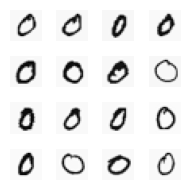
\includegraphics[width=0.8\linewidth]{ps3_ann/30_zeros.png}
        \caption{Zeros}
        \label{fig:reduced-svd}
    \end{subfigure}%
    \begin{subfigure}{.3\textwidth}
        \centering
        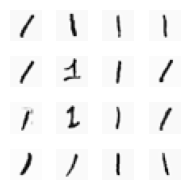
\includegraphics[width=0.8\linewidth]{ps3_ann/31_ones.png}
        \caption{Ones}
        \label{fig:reduced-svd}
    \end{subfigure}%
    \begin{subfigure}{.3\textwidth}
        \centering
        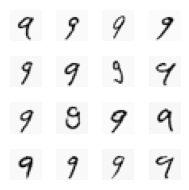
\includegraphics[width=0.8\linewidth]{ps3_ann/32_nines.png}
        \caption{Nines}
        \label{fig:reduced-svd}
    \end{subfigure}%
\caption{Samples from the MNIST dataset}
\label{fig:test}
\end{figure}

Each of the pixel values has a range of [-0.131, 1.127] where most of the values are around 0, and the actual digits' pixels are represented by the values from around 0.1 to 1.

\subsubsection{Initial Training}

The first instance of the model training were done with the following hyperperameters
\begin{verbatim}
    network_a_hyperparams = {
        "layer_sizes": [400, 25, 10],
        "eta": 0.12,
        "epochs": 100,
        "mini_batch_size": 12,
    }
\end{verbatim}

\begin{figure}[h!]
\centering
    \begin{subfigure}{.45\textwidth}
        \centering
        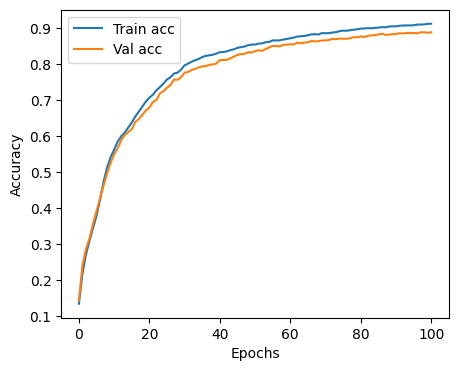
\includegraphics[width=0.98\linewidth]{ps3_ann/02_b_initial_acc.png}
        \caption{Accuracy}
        \label{fig:reduced-svd}
    \end{subfigure}%
    \begin{subfigure}{.45\textwidth}
        \centering
        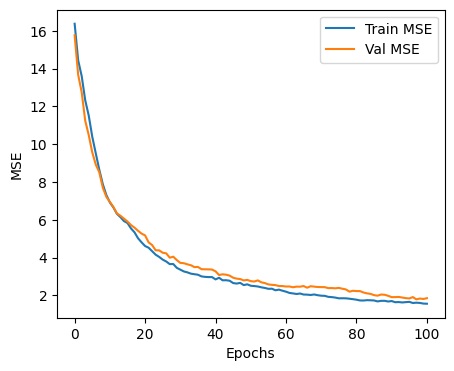
\includegraphics[width=0.98\linewidth]{ps3_ann/02_initial_mse.png}
        \caption{MSE}
        \label{fig:reduced-svd}
    \end{subfigure}%
\caption{Training curves for the initial network}
\label{fig:02_init_net_a_perf}
\end{figure}

\autoref{fig:02_init_net_a_perf} shows the mean squared error training curves for the initial training of the neural network. The curves exhibit an overall logarithmic increase as the number of epochs increase.

Training started with a training accuracy of 0.135, a validation accuracy of 0.144 and an MSE of 16.382 and exihibited a fairly rapid increase in performance from around 0-25 epochs. At the end of the training, the neural network was able to achieve a training accuracy of 0.911, a validation accuracy of 0.888 and an MSE of 1.552.



The first instance of training indicated a slow convergence towards a specific MSE or accuracy value, indicating some of the hyperparameters might need tuning (especially the learning rate eta).

\autoref{fig:02c_init_rep} shows a plot of the final weights connecting the input to the first hidden layer, representing the features that it has learned over training. Note that in this case, the initial training has resulted in a plot that's close to random noise albeit with a few spots that seem to incidate features. In general, the lack of discernable features indicates that the network hasn't been trained enough yet to be able to detect image features through its weight. 

\begin{figure}[h!]
    \centering
    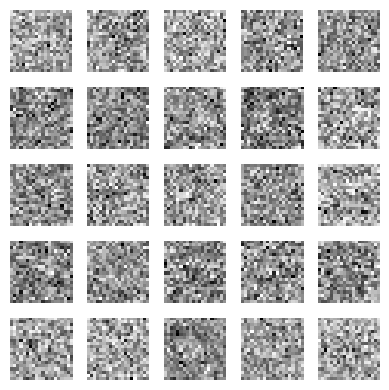
\includegraphics[width=0.35\linewidth]{ps3_ann/02_c_initial_learned_rep.png}
    \caption{Learned Representations for the initial network}
    \label{fig:02c_init_rep}
\end{figure}

\subsubsection{Hyperparameter tuning and further Optimizations}

After some exploration of the network's hyperparameters, another instance of the multilayer perceptron class was created with the following hyperparameters

\begin{verbatim}
    network_c_hyperparams = {
        "layer_sizes": [400, 25, 10],
        "eta": 0.4,
        "epochs": 100,
        "mini_batch_size": 8,
    }
\end{verbatim}
resulting in a significant decrease in required training time (in number of epochs), enabling the network to attain higher performance metrics and attaining satisfactory performance in much fewer epochs.

This new network also includes changes in the way it initializes its weights and biases wherein instead of simply using the standard normal distribution, we normalize the distribution by the square root of the number of weights. These new changes have resulted in the network achieving much better performance when compared to the initial network, where this new network (at the end of the training run) was able to achieve a training accuracy of 0.983 and a validation accuracy of 0.932 (compared to 0.911 and 0.888 for the initial network).

\begin{figure}[h!]
\centering
    \begin{subfigure}{.5\textwidth}
        \centering
        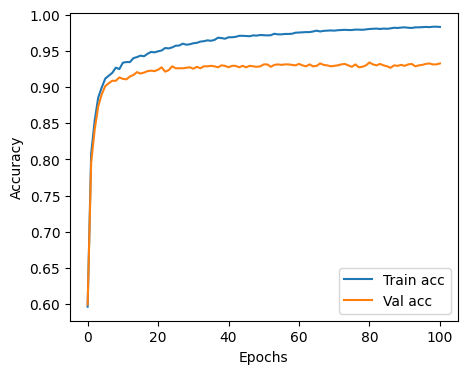
\includegraphics[width=0.9\linewidth]{ps3_ann/08_netc_acc.png}
        \caption{Accuracy}
        \label{fig:reduced-svd}
    \end{subfigure}%
    \begin{subfigure}{.5\textwidth}
        \centering
        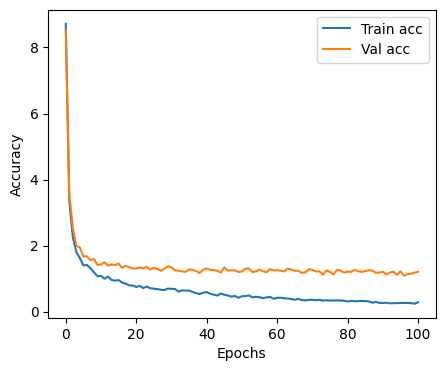
\includegraphics[width=0.9\linewidth]{ps3_ann/09_netc_mse.png}
        \caption{MSE}
        \label{fig:reduced-svd}
    \end{subfigure}%
\caption{Training curves for the new network}
\label{fig:netc_curves}
\end{figure}

\autoref{fig:netc_curves} shows the plot of the training curves for the improved network where with the new settings, the network as already capable of performing at around 0.9 accuracy with as little as 5 epochs. It should be noted however that around 20-25 epochs, validation accuracy starts to plateau while training accuracy still increases, indicating the start of overfitting. One solution for this would be to adopt early stopping, or to simply save the weights at that point.

\begin{figure}[h!]
\centering
    \begin{subfigure}{.5\textwidth}
        \centering
        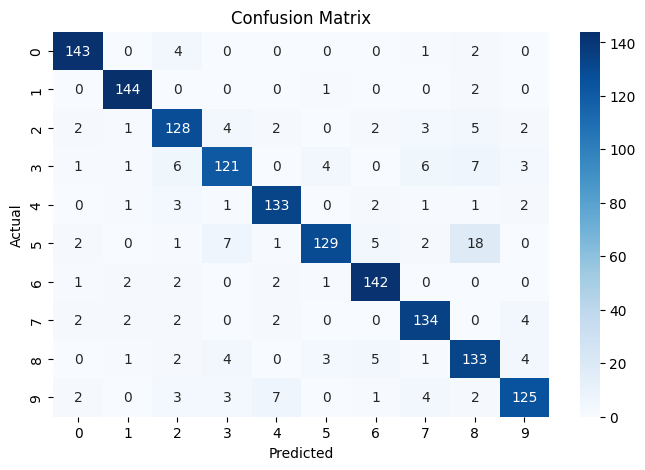
\includegraphics[width=0.95\linewidth]{ps3_ann/02_d_initial_conf.png}
        \caption{Initial Network}
    \end{subfigure}%
    \begin{subfigure}{.5\textwidth}
        \centering
        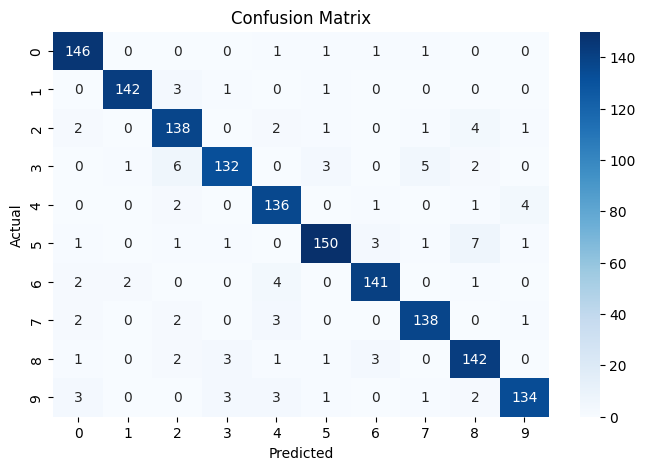
\includegraphics[width=0.95\linewidth]{ps3_ann/10_netc_conf.png}
        \caption{Improved Network}
    \end{subfigure}%
\caption{Before and After Confusion Matrix}
\label{fig:netc_conf}
\end{figure}

\autoref{fig:netc_conf} shows a plot of the confusion matrix for the improved network where we see that the new network has less misclassifications.


\begin{figure}[h!]
    \centering
    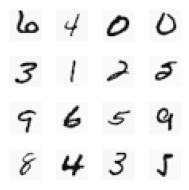
\includegraphics[width=0.20\linewidth]{ps3_ann/11_netc_random_test.png}
    \caption{Random sample images for testing}
    \label{fig:netc_random}
\end{figure}

A few test runs were also performed on a small set of 16 samples images shown in \autoref{fig:netc_random} in order to gauge how well this network performs when we use the weights at the end of training vs at around 23 epochs (before overfitting starts).

\begin{verbatim}
            [[6, 4, 0, 0],       [[6, 4, 0, 0],     [[6, 4, 0, 0],
             [3, 1, 2, 2],        [3, 1, 2, 2],      [3, 1, 2, 5],
             [9, 6, 5, 9],        [9, 6, 5, 9],      [9, 6, 5, 9],
             [8, 4, 3, 3]]        [8, 4, 3, 5]]      [8, 4, 3, 5]]
\end{verbatim}  
The matrices above represent the results of the predictions vs their actual class labels. The matrix on the left accounts for the predictions of the network where the weights used are the final weights at the end of training. The matrix in the middle is for the network where the weights used are at around the 23rd epoch. The matrix on the right are the actual class labels. It can be noted that both versions predicted the "5" that looked a bit like a "2" as a "2", while the overtrained version misclassified the last "5" as a "3".

\begin{figure}[h!]
    \centering
    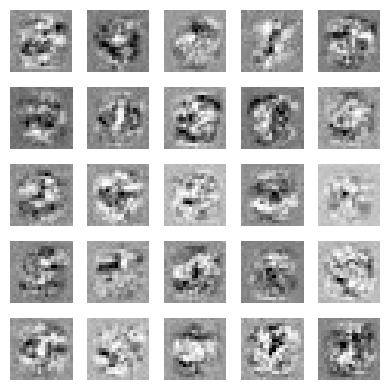
\includegraphics[width=0.45\linewidth]{ps3_ann/12_netc_learned_rep.png}
    \caption{Learned Features for the Improved Network}
    \label{fig:netc_learned_rep}
\end{figure}

\autoref{fig:netc_learned_rep} shows a plot of the weights from the input layer to the hidden layer. In contrast to the initial network, this version shows more distinct patterns which appear to attempt to capture certain features of the numbers. It can also be seen that all of the plots have some sort of mask forming something something like a circle or oval that indicates that the network has learned to focus on the central parts of the image where the digits actually are.

\begin{figure}[h!]
\centering
    \begin{subfigure}{.33\textwidth}
        \centering
        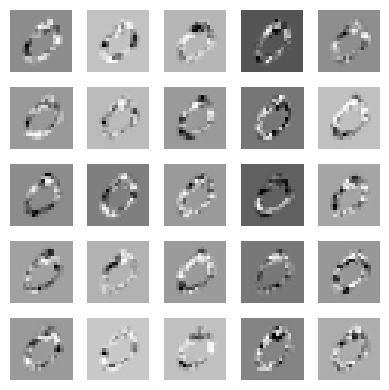
\includegraphics[width=0.95\linewidth]{ps3_ann/13_netc_mask1.png}
        \caption{Example 0 digit}
        \label{fig:exam_0}
    \end{subfigure}%
    \begin{subfigure}{.33\textwidth}
        \centering
        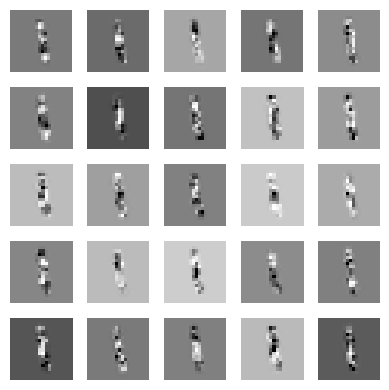
\includegraphics[width=0.95\linewidth]{ps3_ann/14_netc_mask2.png}
        \caption{Example 1 digit}
        \label{fig:exam_1}
    \end{subfigure}%
    \begin{subfigure}{.33\textwidth}
        \centering
        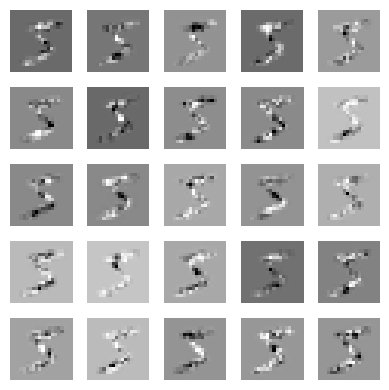
\includegraphics[width=0.95\linewidth]{ps3_ann/15_netc_mask3.png}
        \caption{Example 5 digit}
        \label{fig:exam_2}
    \end{subfigure}%
\caption{Weights applied to example digits}
\label{fig:netc_masks}
\end{figure}

Lastly, \autoref{fig:netc_masks} shows a plot of the same weights shown in \autoref{fig:netc_learned_rep}, except applied to three example digits. \autoref{fig:exam_0} is the same "0" multiplied by the 400 weights for all of the 25 neurons in the hidden layer. \autoref{fig:exam_1} is the same number "1" applied to the same weights, etc.

When viewed from this perspective, the weights seem to capture certrain geometric patterns such as loops, lines, positions of pixels, horizontal patterns, diagonal patterns, etc. For example, take a look at the middle tile for the lowest row of all the three figures. Notice how the all seem to capture the extreme ends of each number. For example, it captures the upper and lower parts of the "0" digit, and the same goes for the "1" and "5" digit. Another would be the first tile of the middle row, which seems to be responsible for detecting a lower diagonal (notice the "0" and the "5").

These patterns are then fed to the output (or any subsequent hidden) layers which then make more fine-tuned decisions based on these patterns in order to make a prediction.




% -------------------
% -------------------
% -------------------
% -------------------
% -------------------

\pagebreak

\section{Hybrid Optimization}
\subsection{Understanding of the Problem}
    \subsubsection{Motivation}
        Having to learn by application is a blessing for us. Early in this MEng in AI program, exposure to these types of problems can provide us an opportunity to increase our understanding of the fundamentals and theoretical foundations of AI, which will serve as a good starting point for our upcoming advanced courses. Since optimization is a cornerstone of machine learning, it plays a critical role in enhancing the performance and accuracy of models. Optimization involves adjusting the parameters of a model to minimize or maximize an objective function, which often corresponds to reducing errors or improving predictions. Effective optimization ensures that a machine learning model can learn from data efficiently, generalize well to new, unseen data, and ultimately make accurate predictions. 

        Given the complexity and variety of machine learning problems, hybrid optimization approaches, which combine the strengths of different optimization methods, are becoming increasingly vital. Traditional optimization techniques, such as gradient descent, might struggle with non-convex or highly irregular objective landscapes, while heuristic or metaheuristic methods, like genetic algorithms or particle swarm optimization, offer powerful alternatives but can be computationally expensive. By integrating these methods, hybrid optimization leverages the precision and speed of traditional algorithms with the flexibility and robustness of heuristic approaches. This synergy not only enhances the convergence rate and solution quality but also broadens the applicability of optimization techniques to a wider range of machine learning problems. Consequently, hybrid optimization stands as a promising direction to address the diverse challenges in machine learning, leading to more reliable, efficient, and adaptable models.

    \subsubsection{Statement of the Problem}
        The problem of inefficiency and limitations from current optimization techniques in effectively training machine learning models, particularly when dealing with complex, non-convex, or highly irregular objective functions. Traditional optimization methods often face challenges in convergence and can easily get trapped in local minima, while heuristic methods, although flexible, are computationally intensive and not always practical for large-scale problems. This necessitates the development of hybrid optimization approaches that can leverage the strengths of multiple methods to achieve more reliable, efficient, and accurate optimization in machine learning. The goal is to create a robust optimization framework that enhances model performance across diverse applications and scales.

        For this specific paper, we will examine how two optimization algorithms compare with our hybrid optimization algorithm across various metrics.

\subsection{Methodology and Snapshots of the Solution}
    \subsubsection{Overview of the Methodology}
        
        The proposed hybrid optimization method is designed to optimize the Bohachevsky function by effectively combining the strengths of the Steepest Descent method with Armijo's Rule and Newton's Method with Trust Region. Initially, the algorithm employs the Steepest Descent method with Armijo's Rule to make rapid progress in the early stages of optimization. This approach ensures that the algorithm efficiently navigates the steep slopes of the objective function, making significant strides towards reducing the objective function value. Armijo's Rule is used to adaptively adjust the step size, balancing the need for large steps to expedite progress and small steps to avoid overshooting.
        
        As the optimization progresses and the algorithm approaches regions where the gradient norms are smaller, it transitions to Newton's Method with a Trust Region approach. This shift leverages the quadratic convergence properties of Newton's Method, allowing for more precise adjustments to the parameter values in these flatter regions. The Trust Region approach is incorporated to ensure robustness, preventing large, potentially destabilizing steps by restricting the step size to within a manageable "trust region" around the current point. The convergence criteria for this hybrid method involve checking the gradient norm, ensuring that the algorithm continues iterating until the gradient norm falls below a predetermined threshold, indicating that an optimal or near-optimal solution has been found. This hybrid strategy balances the rapid initial convergence with the precision required for final fine-tuning, making it effective for optimizing complex functions like the Bohachevsky function.

    \subsubsection{Bohachevsky Function}
        The Bohachevsky Function 1st variant is a commonly used test function in optimization, notable for its simplicity yet challenging landscape. The function is defined as:
        \[
            f_1(x,y) = x^2 + 2y^2 - 0.3cos(3\pi x) - 0.4cos(4 \pi y) + 0.7
        \]

        The surface of the function shown in \autoref{fig:Bolchesvsky} is characterized by a parabolic bowl shape with added sinusoidal ripples, creating multiple local minima and maxima:
        
        \begin{figure}[h!]
            \centering
            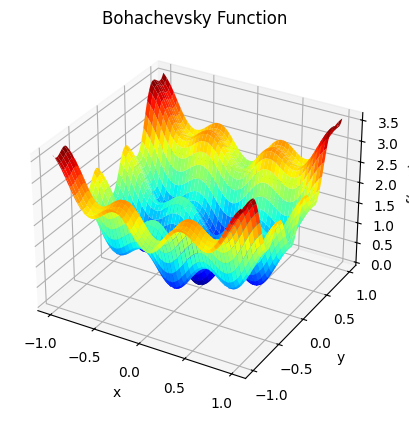
\includegraphics[width=0.43\linewidth]{ps4_hybrid/bohachevsky.png}
            \caption{Bolchesvsky Function}
            \label{fig:Bolchesvsky}
        \end{figure}

        These features make the Bohachevsky Function an excellent benchmark for evaluating the performance of optimization algorithms, particularly in terms of their ability to navigate and escape local minima to find the global minimum.
    \subsubsection{Gradient and Hessian of Bohachevsky Function}
        The gradient and Hessian of the Bohachevsky function \( f_1(x, y) \) are derived through calculus, specifically partial differentiation.
        \begin{itemize}
            \item The gradient is a vector of the first partial derivatives of the function with respect to \(x\) and \(y\):
            \begin{enumerate}
                \item Partial derivative with respect to \(x\):
                \[ \frac{\partial f_1}{\partial x} = \frac{\partial}{\partial x} \left( x^2 + 2y^2 - 0.3 \cos(3\pi x) - 0.4 \cos(4\pi y) + 0.7 \right) \]
                \[ \frac{\partial f_1}{\partial x} = 2x + 0.9\pi \sin(3\pi x) \]
                \item Partial derivative with respect to \(y\)
                \[ \frac{\partial f_1}{\partial y} = \frac{\partial}{\partial y} \left( x^2 + 2y^2 - 0.3 \cos(3\pi x) - 0.4 \cos(4\pi y) + 0.7 \right) \]
                \[ \frac{\partial f_1}{\partial y} = 4y + 1.6\pi \sin(4\pi y) \]
            \end{enumerate}
    
                So, the gradient \( \nabla f_1(x, y) \) is:
                \[ \nabla f_1(x, y) = \left[ \frac{\partial f_1}{\partial x}, \frac{\partial f_1}{\partial y} \right] = \left[ 2x + 0.9\pi \sin(3\pi x), 4y + 1.6\pi \sin(4\pi y) \right] \]

            \item The Hessian matrix is a square matrix of the second partial derivatives of the function:
            \begin{enumerate}
                \item Second partial derivative with respect to \( x \):
                \[ \frac{\partial^2 f_1}{\partial x^2} = \frac{\partial}{\partial x} \left( 2x + 0.9\pi \sin(3\pi x) \right) \]
                \[ \frac{\partial^2 f_1}{\partial x^2} = 2 + 2.7\pi^2 \cos(3\pi x) \]
                \item Second partial derivative with respect to \( y \)
                \[ \frac{\partial^2 f_1}{\partial y^2} = \frac{\partial}{\partial y} \left( 4y + 1.6\pi \sin(4\pi y) \right) \]
                \[ \frac{\partial^2 f_1}{\partial y^2} = 4 + 6.4\pi^2 \cos(4\pi y) \]
                \item Mixed second partial derivatives:
                \[ \frac{\partial^2 f_1}{\partial x \partial y} = \frac{\partial^2 f_1}{\partial y \partial x} = 0 \]
                
            \end{enumerate}
                So, the Hessian matrix \( H \) is:
                \[ H = \begin{bmatrix} \frac{\partial^2 f_1}{\partial x^2} & \frac{\partial^2 f_1}{\partial x \partial y} \\ \frac{\partial^2 f_1}{\partial y \partial x} & \frac{\partial^2 f_1}{\partial y^2} \end{bmatrix} = \begin{bmatrix} 2 + 2.7\pi^2 \cos(3\pi x) & 0 \\ 0 & 4 + 6.4\pi^2 \cos(4\pi y) \end{bmatrix} \]
        \end{itemize}
    \subsubsection{Trust Region Newton method}

    Newton's method with trust region is an iterative optimization technique used to find a local minimum of a continuously differentiable function \( f : \mathbb{R}^n \to \mathbb{R} \). Unlike the basic Newton's method, which uses a quadratic approximation to the objective function and updates the solution based on the Hessian matrix, the trust region approach modifies this by limiting the step size to stay within a certain "trust region". This is particularly useful when the quadratic model is not a good approximation of the objective function far from the current point. At each iteration \( k \), the method solves a subproblem that minimizes the quadratic model of \( f \) within a ball of radius \( \Delta_k \) centered at the current point \( x_k \). This ensures that the steps taken are controlled, reducing the risk of making large, potentially harmful steps.

    The methodology is outlined in pseudocode as follows: starting at an initial point \( x_0 \), the goal is to construct a sequence of iterates \( \{ x_k \} \) such that \( f(x_{k+1}) < f(x_k) \) for all \( k \geq 0 \), unless \( x_k \) is optimal. At each iteration, the algorithm approximates \( f \) by a quadratic model \( m_k(d) = f(x_k) + \nabla f(x_k)^T d + \frac{1}{2} d^T B_k d \), where \( \nabla f(x_k) \) is the gradient and \( B_k \) is an approximation to the Hessian matrix. The step \( d_k \) is found by approximately solving the trust region subproblem:
    
    \begin{align*}
        \min_{d} \quad & m_k(d) \\
        \textrm{subject to} \quad  & \|d\| \leq \Delta_k.
    \end{align*}
    
    The trust region radius \( \Delta_k \) is adjusted based on how well the quadratic model predicts the actual reduction in \( f \). If the predicted reduction is accurate, \( \Delta_k \) may be increased; otherwise, it is decreased. The new point is then updated as \( x_{k+1} = x_k + d_k \). The process continues until convergence criteria are met, such as a sufficiently small gradient or a maximum number of iterations.
    
    \subsubsection{Steepest Descent method}
    
    Given a continuously differentiable (loss) function \(f : R^n \to R \), steepest descent is an iterative procedure to find a local minimum of \(f\) by moving in the opposite direction of the gradient of \(f\) at every iteration \(k\).

    Steepest descent is summarized below in a pseudocode where \(\epsilon_k\) is the stepsize parameter at iteration \(k\). \(\epsilon_k\) is sometimes called learning rate
    in the context of machine learning. 
    
    Starting at some \(x_0 \in X\), the goal of the iterative scheme is to construct a sequence of iterates \(\{ x_k \} \subset X\) such that
    \[f(x_k+1) < f(x_k), \forall k \geq 0,\]
    unless \(x_k\) is optimal in which case the algorithm terminates. It is now useful to consider the directional derivative of \(f\) at a point \(x\) in a direction \(d\), defined as follows:
    \[\Delta_d f(x) = \lim_{\epsilon \to 0} \frac{f(x + \epsilon d) - f(x)}{\epsilon }\]

    For a differentiable \(f\):
    \[\Delta_d f(x) = \Delta f(x)^T d\]

    From this formula it follows that if \(d_k\) is a descent direction at \(x_k\) in the sense that
    \[\Delta f(x_k)^T d_k < 0,\]

    then we may reduce \(f\) by moving from \(x_k\) along \(d_k\) with a sufficiently small positive stepsize \(\epsilon\). In the unconstrained case where \(X = \mathbf{R}^n\)
    this leads to the gradient descent scheme where \(d_k\) is a descent direction at \(x_k\) and \(\epsilon_k\) is a positive scalar stepsize.
    
    If \(d_k = -\Delta f(x_k)\), then the gradient descent algorithm becomes the steepest descent.

    Below is the pseudocode for the Steepest Descent Method:
    \begin{verbatim}
        def steepest_descent(f, grad_f, x0, tol=1e-6, max_iter=1000):
            x_k = np.array(x0)
            for k in range(max_iter):
                grad_k = grad_f(x_k)
                if np.linalg.norm(grad_k) < tol:
                    break
                d_k = -grad_k
                epsilon_k = 1   ## change this to Armijo
                x_k = x_k + epsilon_k * d_k
            return x_k, f(x_k)

        # Example usage
        # f: objective function
        # grad_f: gradient of the objective function
        # epsilon0: initial stepsize
        # x0: initial point
        # tol: tolerance (e.g., 1e-6)
        # max_iter: maximum iterations (e.g., 1000)
    \end{verbatim}

    Notice that we set \(\epsilon_k\) as constant or commonly called as Fixed Stepsize:
    \[\epsilon_k = \epsilon, \forall k \geq 0\]
    
    But there are many ways we can define the stepsize \(\epsilon_k\). But we will be focusing on Armijo's Rule.

    \subsubsection{Armijo's Rule}
    
    Armijo rule, also known as backtracking line search, ensures that the (loss) function \(f\) decreases sufficiently at every iteration. In return, it reduces complexity as compared to optimal line search. To understand how the Armijo rule works, we may use Taylor’s theorem to write:
    \begin{align*}
        f(x_k + \epsilon d_k) &= f(x_k) + \Delta f(x_k)^T(x_k + \epsilon d_k - x_k) + o(||x_k + \epsilon d_k - x_k||)\\
        &= f(x_k) + \epsilon \Delta f(x_k)^T d_k + o(\epsilon)
    \end{align*} 

    If \(\epsilon\) is sufficiently small, then the term \(\epsilon |\Delta f(x_k)^T d_k|\) becomes dominant compared to \(o(\epsilon)\). Also, \(\epsilon \Delta f(x_k)^T d_k < 0\), since \(d_k\) is a descent direction at \(x_k\). As a result,
    \[f(x_k + \epsilon d_k) = f(x_k).\]

    Hence, at every iteration, the Armijo rule attempts to pick a sufficiently small \(\epsilon\). In summary, at iteration \(k\) of the steepest gradient descent algorithm:

    \begin{enumerate}[label=(\roman*)]
        \item Start with \(\epsilon = \epsilon_0\) for some pre-selected \(\epsilon_0\). Let \(0 < \sigma < 1, 0<\beta<1\) be two user-defined parameters.
        \item If \(f(x_k + \epsilon d_k) \leq f(x_k) + \sigma \epsilon \Delta f(x_k)^T d_k,\) stop and return the current value of \(\epsilon,\) else set \(\epsilon \leftarrow  \beta \epsilon \) and repeat step (ii).
    \end{enumerate}

    Thus, the Armijo rule terminates at the first iteration \(l \geq 1\)  such that
    \[f(x_k + \beta^l\epsilon_0 d_k) = f(x_k) + \sigma \beta^l \epsilon_0 \Delta f(x_k)^T d_k\]


    Below is the pseudocode for Armijo rule:
    \begin{verbatim}
        def armijo_rule(f, grad_f, x, d_k, epsilon_0=1, beta=0.5, sigma=10**(-4)):
            fx = f(x[0], x[1])
            grad_fx = grad_f(x[0], x[1])
            epsilon = epsilon_0
            while True:
                if f(x[0] + epsilon * d_k[0], x[1] + epsilon * d_k[1]) <= 
                        fx + sigma * epsilon * np.dot(grad_fx, d_k):
                    break
                epsilon *= beta
            return epsilon

        # Example usage
        # f: objective function
        # grad_f: gradient of the objective function
        # x: point (x,y)
        # epsilon0: initial stepsize
        # beta: 1/2 to 1/10 (standard practice)
        # sigma: sigma in [10^-5, 10^-1] (standard practice)
        # max_iter: maximum iterations (e.g., 1000)
    \end{verbatim}

    
    We can now insert this pseudocode to our steepest descent code by changing:
    \begin{verbatim}
        epsilon_k = epsilon0 
        to 
        epsilon_k = armijo_rule(f, grad_f, x, d_k)
    \end{verbatim}

    \subsubsection{Hybrid Method}
    The hybrid optimization method combines the strengths of Newton's method with trust region and the steepest descent method with Armijo's rule. The process begins with an initial point \( x_0 = [1.5, 1.5] \) and a predefined step size parameter \( \epsilon = 0.3 \). The first iteration employs Newton's method with a trust region approach to take an initial step. Specifically, the trust region method constructs a quadratic model of the objective function and solves the trust region subproblem to determine an optimal step direction and length within a predefined region. This step ensures that the algorithm starts with a well-informed direction, balancing rapid convergence near the optimal point with stability.

    After the initial step using Newton's method with trust region, the algorithm switches to the steepest descent method with Armijo’s rule for subsequent iterations. The steepest descent method involves moving in the direction opposite to the gradient of the function. Armijo's rule is employed to adaptively determine the step size, ensuring sufficient decrease in the function value at each step. This rule modifies the step size \( \epsilon_k \) dynamically to guarantee that the descent condition \( f(x_k + \epsilon_k d_k) \leq f(x_k) + c \epsilon_k \nabla f(x_k)^T d_k \) is satisfied, where \( d_k = -\nabla f(x_k) \) and \( c \) is a predefined constant in \( (0, 1) \). The iterative process of steepest descent continues until convergence criteria, such as a sufficiently small gradient norm or a maximum number of iterations, are met. This hybrid approach leverages the fast convergence properties of Newton’s method initially and the robustness and simplicity of steepest descent for further refinement.
    
\subsection{Results, Analysis and Discussion}
    \subsubsection{Optimization Result}
    The plot and the evaluation data provided a comparative analysis of three optimization methods applied to the Bohachevsky function (first function):
    \begin{itemize}
        \item Trust Region Newton method
        \item Steepest Descent with Armijo's Rule
        \item Hybrid Method
    \end{itemize}

    The results demonstrate the performance and efficiency of each method in terms of path taken, computation time, and the number of function and gradient evaluations.
    
    \begin{figure}[h!]
        \centering
        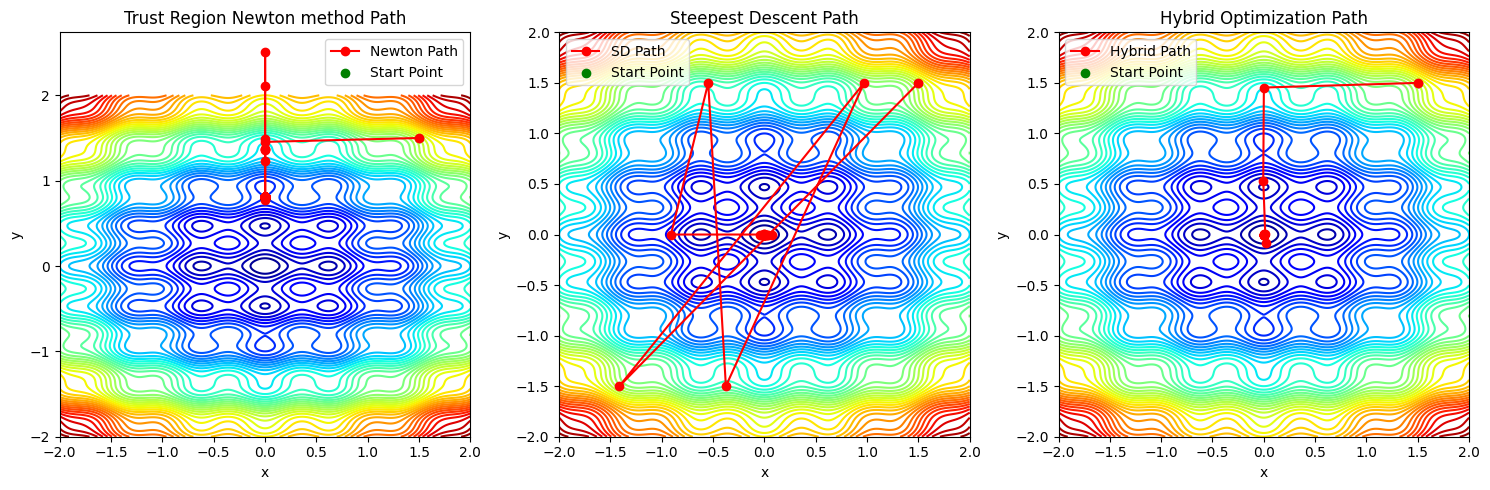
\includegraphics[width=1\linewidth]{ps4_hybrid/hybrid.png}
    \end{figure}
    
    \begin{figure}[h!]
        \centering
        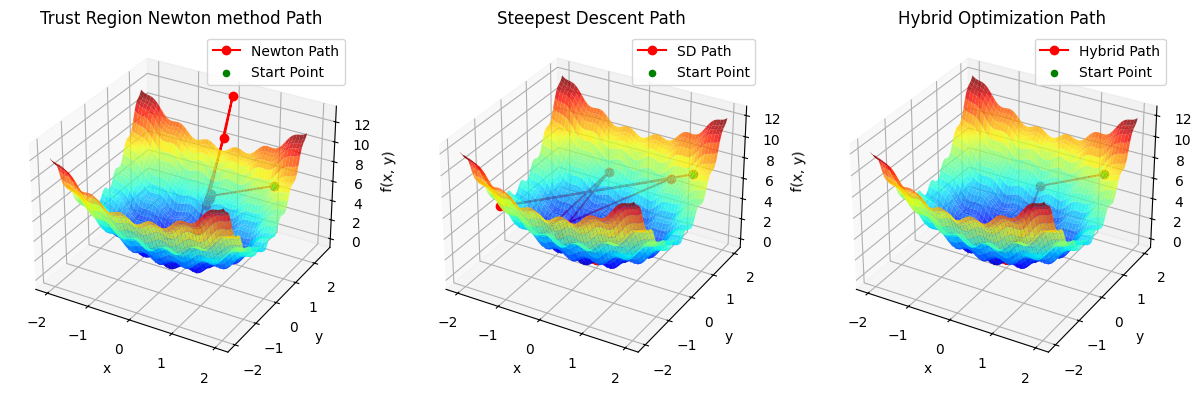
\includegraphics[width=1\linewidth]{ps4_hybrid/3d hybrid.png}
    \end{figure}

    \begin{table}[h!]
    \centering
    \caption*{Comparison of Optimization Methods}
    \begin{tabular}{lcccc}
    \toprule
    \textbf{Method} & \textbf{Time (s)} & \textbf{Function Evaluations} & \textbf{Gradient Evaluations} \\
    \midrule
    Trust Region Newton method & 0.0385980 & 1000 & 1000 \\
    Steepest Descent with Armijo's Rule & 0.0007537 & 26 & 27 \\
    Hybrid Method & 0.0004345 & 16 & 17 \\
    \bottomrule
    \end{tabular}
    \label{tab:comparison}
    \end{table}

    \newpage
    To improve the optimization process further, the following enhancements could be considered:

    \begin{enumerate}
        \item Adaptive Trust Region Radius: Implementing an adaptive mechanism to adjust the trust region radius dynamically based on the optimization progress can enhance the performance of the Newton with Trust Region method.
        \item Hybrid Strategy Tuning: Fine-tuning the transition point and criteria between the Newton and steepest descent methods could further optimize the hybrid method, potentially reducing the number of function and gradient evaluations.
        \item Parallel Computing: Leveraging parallel computing techniques can significantly reduce computation time, especially for methods with high function and gradient evaluations.
        \item Adaptive Step Size in Hybrid Method: Introducing an adaptive step size mechanism within the hybrid method, similar to Armijo's rule, could balance the benefits of both methods more effectively.
    \end{enumerate}
    
    Overall, the hybrid method shows promising results with the fastest convergence and the least computational effort among the three methods. Further refinement and enhancements can make it even more robust and efficient for various optimization problems.

\end{document}
